%\documentclass[aps,prx,superscriptaddress, nofootinbib]{revtex4-2}%Use revtex4-2
\documentclass[aps,prx,twocolumn,notitlepage,nofootinbib,nobalancelastpage]{revtex4-2}
\pdfoutput=1

\usepackage[T1]{fontenc}
\usepackage{amsmath,amsfonts,amssymb,amsthm,bbm,bm, braket}
\usepackage{wasysym}
\usepackage{comment}
\usepackage{scalerel}
\usepackage{enumerate}
\usepackage{amssymb}
\usepackage{graphicx}
\usepackage{mathtools}
\usepackage{ifthen}
\usepackage{tensor}
\usepackage{tikz}
\usepackage{tikz-network}
%\usetikzlibrary{shapes.geometric}%added
\usetikzlibrary{patterns,decorations.pathreplacing}

\usepackage{color}
\usepackage{longtable}%Added!
\usepackage[normalem]{ulem} % either use this (simple) 

\theoremstyle{break}        
\newtheorem{Prop}{Property} %\newtheorem{Prop}{Property}[section]
\newtheorem{Lemma}{Lemma}
%\newtheorem{Lemma}{Lemma}[section]
\newtheorem{Proposition}{Proposition}
%\newtheorem{Proposition}{Proposition}[section]
\usepackage{color}
\definecolor{myred}{RGB}{232,102,102}
\definecolor{myblue}{RGB}{187,187,255}
\definecolor{myorange0}{RGB}{252,226,5}
\definecolor{myorange0c}{RGB}{255,255,255}
\definecolor{myorange}{RGB}{255,165,0}
\definecolor{mygrey}{RGB}{105,105,105}
\definecolor{OliveGreen}{RGB}{85,107,47}
\definecolor{NavyBlue}{RGB}{0,0,128}
%\definecolor{myY}{RGB}{220,255,203}
\definecolor{mygreen}{RGB}{34,139,34}
\definecolor{myY}{RGB}{220,255,203}
\definecolor{myYO}{RGB}{255, 220, 151}

\definecolor{mygreenc}{RGB}{150,50,50}

\usepackage{tensor}
\newcommand{\be}{\begin{equation}}
\newcommand{\ee}{\end{equation}}
\newcommand{\ba}{\begin{aligned}}
\newcommand{\ea}{\end{aligned}}
\newcommand{\bw}{\begin{widetext}}
\newcommand{\ew}{\end{widetext}}
\newcommand{\1}{\mathbbm{1}}
\newtheorem{theorem}{Theorem}
\theoremstyle{plain}
\newtheorem{property}{Property}
\theoremstyle{plain}
\newtheorem{lemma}{Lemma}
\theoremstyle{plain}
\newtheorem{observation}{Observation}
\usepackage[colorlinks,bookmarks=false,citecolor=NavyBlue,linkcolor=OliveGreen,urlcolor=blue]{hyperref}




\DeclareMathOperator{\arccosh}{arcCosh}
\newcommand{\du}{{\rm du}}

\renewcommand{\qedsymbol}{$\blacksquare$}

\newcommand{\Wgatedagger}[2]{
\draw[very thick] (#1-0.5, #2 +0.5) -- (#1+0.5,#2-0.5);
\draw[very thick] (#1-0.5,#2-0.5) -- (#1+0.5,#2+0.5);
\draw[ thick, fill=mygreenc, rounded corners=2pt] (#1-0.25,#2+0.25) rectangle (#1+0.25,#2-0.25);
\draw[thick] (#1,#2+0.15) -- (#1+0.15,#2+0.15) -- (#1+0.15,#2);
%\Text[x=0,y=-0.075]{\x \y}
}
\newcommand{\Wgatered}[2]{
\draw[very thick] (#1-0.5, #2 +0.5) -- (#1+0.5,#2-0.5);
\draw[very thick] (#1-0.5,#2-0.5) -- (#1+0.5,#2+0.5);
\draw[ thick, fill=myred, rounded corners=2pt] (#1-0.25,#2+0.25) rectangle (#1+0.25,#2-0.25);
\draw[thick] (#1,#2+0.15) -- (#1+0.15,#2+0.15) -- (#1+0.15,#2);
%\Text[x=0,y=-0.075]{\x \y}
}
\newcommand{\Wgateblue}[2]{
\draw[very thick] (#1-0.5, #2 +0.5) -- (#1+0.5,#2-0.5);
\draw[very thick] (#1-0.5,#2-0.5) -- (#1+0.5,#2+0.5);
\draw[ thick, fill=myblue, rounded corners=2pt] (#1-0.25,#2+0.25) rectangle (#1+0.25,#2-0.25);
\draw[thick] (#1,#2+0.15) -- (#1+0.15,#2+0.15) -- (#1+0.15,#2);
%\Text[x=0,y=-0.075]{\x \y}
}
\newcommand{\Wgategreen}[2]{
\draw[very thick] (#1-0.5, #2 +0.5) -- (#1+0.5,#2-0.5);
\draw[very thick] (#1-0.5,#2-0.5) -- (#1+0.5,#2+0.5);
\draw[ thick, fill=mygreen, rounded corners=2pt] (#1-0.25,#2+0.25) rectangle (#1+0.25,#2-0.25);
\draw[thick] (#1,#2+0.15) -- (#1+0.15,#2+0.15) -- (#1+0.15,#2);
%\Text[x=0,y=-0.075]{\x \y}
}
\newcommand{\MYcircle}[2]{
\draw[thick, fill=white] (#1,#2) circle (0.1cm); }
\newcommand{\MYsquare}[2]{
%\node[regular polygon,
%    draw= thick,
%    regular polygon sides = 4,
 %    fill =white,
 %    minimum size = .2cm
 %    ] (p) at (#1,#2) {}; 
 \coordinate (Origin) at (#1,#2);
\filldraw [thick, fill=white, even odd rule] ($(Origin)+(-.1cm,-.1cm)$) coordinate (Square) -- ++(0.0cm,0.2cm) -- ++(0.2cm,0.0cm) -- ++(0.0cm,-0.2cm) -- cycle;
 }
\newcommand{\MYtriangle}[2]{
 \coordinate (Origin) at (#1,#2);
\filldraw [thick, fill=white, even odd rule] ($(Origin)+(-.0cm,{0.666*cos(60)*0.3cm})$) coordinate (Triangle) -- ++(0.15cm,-{cos(60)*0.3cm}) -- ++(-0.3cm,0.0cm) -- ++(0.15cm,{cos(60)*0.3cm}) -- cycle;
}
\newcommand{\MYcircleB}[2]{
\draw[thick, fill=black] (#1,#2) circle (0.1cm); }

\newcommand{\rhoO}[2]{
\draw[very thick] (-.5+#1,0.5+#2) -- (#1,0+#2);
\draw[very thick] (#1,0+#2) -- (.5+#1,0.5+#2);
\draw[very thick] (-.5+#1,#2) -- (.5+#1,#2);
\draw[ thick, fill=mygreen, rounded corners=2pt] (-0.35+#1,0.2-0.25+#2) rectangle (0.35+#1,0.2+0.2+#2);
\draw[very thick] (0.1+#1,0.15+.18+#2)-- (.15+0.1+#1,0.15+.18+#2) -- (.15+0.1+#1,0+.18+#2);
}

\newcommand{\Wgategrey}[2]{
\draw[very thick] (#1-0.5, #2 +0.5) -- (#1+0.5,#2-0.5);
\draw[very thick] (#1-0.5,#2-0.5) -- (#1+0.5,#2+0.5);
\draw[ thick, fill=mygrey, rounded corners=2pt] (#1-0.25,#2+0.25) rectangle (#1+0.25,#2-0.25);
\draw[thick] (#1,#2+0.15) -- (#1+0.15,#2+0.15) -- (#1+0.15,#2);
%\Text[x=0,y=-0.075]{\x \y}
}
\newcommand{\mcirc}{\mathbin{\scalerel*{\fullmoon}{G}}}
\newcommand{\msquare}{\mathord{\scalerel*{\Box}{G}}}
\newcommand{\mcircf}{\mathbin{\scalerel*{\newmoon}{G}}}
\newcommand{\mtriangle}{\mathord{\scalerel*{\triangle}{G}}}
\newcommand{\MYsquareB}[2]{

\draw[ thick, fill=black, rounded corners=2pt] (#1-0.25,#2+0.25) rectangle (#1+0.25,#2-0.25);
\draw[thick, color=white] (#1,#2+0.15) -- (#1+0.15,#2+0.15) -- (#1+0.15,#2);
%\Text[x=0,y=-0.075]{\x \y}
}

\newcommand{\tr}{\text{tr} \, }
\newcommand{\Tr}{\text{Tr} \, }
%Tiles
\newcommand{\lineW}{.8mm}
\newcommand{\sroot}{1.41421356237}

%\input{HeadIncludes.txt}
\def\scale{0.3}

\newcommand{\gs}[1]{{\color{red}[#1]}}
\newcommand{\pk}[1]{{\color{blue}[#1]}}
\definecolor{skyblue}{RGB}{135, 206, 235}
%Set up the metadata
\hypersetup{
 pdftitle={Hierarchical generalization of dual unitarity},
 pdfsubject={Many-body systems},
 pdfauthor={Xie-Hang Yu, Xie-Hang Yu, and Pavel Kos},
 pdfkeywords={exact solutions, quantum circuits, quantum many-body systems}
}


\begin{document}

\title{Hierarchical generalization of dual unitarity} 


\author{Xie-Hang Yu}
\author{Zhiyuan Wang}
\author{Pavel Kos}%

\affiliation{Max-Planck-Institut f{\"{u}}r Quantenoptik, Hans-Kopfermann-Str. 1, 85748 Garching, Germany}%
%\affiliation{Munich Center for Quantum Science and Technology (MCQST), Schellingstr. 4, 80799 M{\"{u}}nchen, Germany}%


\date{\today}

\begin{abstract}
Quantum dynamics with local interactions in lattice models display rich physics, but is notoriously hard to study. Dual-unitary circuits allow for exact answers to interesting physical questions in clean or disordered one- and higher-dimensional quantum systems. 
However, this family of models shows some non-universal features, like vanishing correlations inside the light-cone and instantaneous thermalization of local observables.
In this work we propose a generalization of dual-unitary circuits where the exactly calculable spatial-temporal correlation functions display richer behavior, and have non-trivial thermalization of local observables. This is achieved by generalizing the 
single-gate condition to a hierarchy of multi-gate conditions, where the first level recovers dual-unitary models, and the second level exhibits these new interesting features. 
We also extend the discussion and provide exact solutions to correlators with few-site observables and discuss higher-orders, including the ones after a quantum quench. In addition, we provide exhaustive parametrizations for qubit cases, and propose a new family of models for local dimensions larger than two, which also provides a new family of dual-unitary models.
%
%In the second part, we present analytical solutions for these families. 
%Merge to before
%We compute spatio-temporal correlations for $2^{\mathrm{nd}}$ Hierarchicals, showing that they exhibit richer physics than dual-unitary models with nonzero correlations at the same site. Next, we discuss how higher Hierarchicals shrink the light-cone.
%We also extend the discussion to few-site observables and higher-order correlators. Moreover, we discuss the one- and two-point equal-time correlators after a quantum quench, and analytically express the non-trivial thermalization of local observables. 
%
%Our results provide a strong foundation for further explorations of solvable models and their real-world applications.
\end{abstract}
\maketitle

\section{Introduction} \label{sec:Intro}

%Intro paragraph
One of the pivotal problems in quantum many-body physics is understanding the dynamics of extended systems with local interactions. Although the local interactions are simple, they generate complex dynamics, which is in general too hard to describe.
The dynamics can be characterized with different probes such as local correlation functions, entanglement spreading, and other quantum information quantities.
The understanding of this type of dynamics is currently at the center of attention in many fields spanning from nonequilibrium statistical mechanics, quantum information, condensed matter to high-energy physics and quantum gravity.

%Importance of solvable models

%Complexity
However, the complexity of quantum dynamics, both analytically and numerically, presents a significant hurdle. For example, the bond dimension of Matrix Product States (MPS) typically increases exponentially due to the linear growth in entanglement entropy~\cite{Daley2004time,Schuch2008entropy}. 
This necessitates the use of solvable models to unravel many-body behavior. The most well-known examples are noninteracting (Gaussian) systems such as free fermions or bosons, Clifford circuits, and Bethe-ansatz interacting integrable models. 
Unfortunately, all of these models are not chaotic, in contrast to generic examples. 
If one is prepared to average over an ensemble of systems, random unitary circuits~\cite{%nahum2017quantum,nahum2018operator,von2018operator,rakovszky2019sub,chan2018solution,garratt2021local,PhysRevResearch.5.013044
fisher2023random} provide examples of solvable chaotic dynamics. However, the averaged results miss a lot of relevant physics and are less relevant for translationally invariant systems.
%these random ensembles often require intricate artificial designs and are rare in the majority of natural systems which uphold spatial-temporal translational invariance.
%Disadvantage of random unitary: not suitable for describing specific physical systems

%DU paragraphs

A recently discovered solvable family of models, known as \emph{dual-unitary}  quantum circuits~\cite{bertini2019exact}, has distinctly different solvable structure which does not require averaging, and moreover contains both integrable and chaotic examples.
The basic property, which enables solvability is the unitarity of the local gates in the space direction. In this paper, we generalize this to a condition on a few gates and unravel new families of solvable models.

Dual unitarity was shown to enable analytical computations of correlation functions~\cite{bertini2019exact,piroli2020exact},
chaos indicator spectral form factor~\cite{bertini2018exact,bertini2021random}, operator and entanglement spreading~\cite{bertini2019entanglement,bertini2020operator, gopalakrishnan2019unitary, piroli2020exact,claeys2020maximum,bertini2020scrambling, reid2021entanglement, zhou2022maximal}, 
deep thermalization through emergent state designs~\cite{ho2022exact,claeys2022emergent,ippoliti2022dynamical}, study of eigenstate thermalization~\cite{fritzsch2021eigenstate} and
temporal entanglement~\cite{lerose2020influence,Giudice2022temporal, foligno2023temporal}.
They also proved useful in connections with measurement induced phase transitions~\cite{ippoliti2021postselection, ippoliti2021fractal,lu2021spacetime}, had aspects of their computational power characterized~\cite{suzuki2021computational}, and have already been realized in experimental setups~\cite{chertkov2021holographic, mi2021information}. %\pk{I need to think if something is still missing?}
%
%
The exhaustive parametrization is simple and is known for dual-unitary gates of two qubits~\cite{bertini2019exact}.
In general, however, only certain non-exhaustive families of gates are known~\cite{rather2020creating, gutkin2020exact, claeys2021ergodic, aravinda2021from,prosen2021manybody, marton2022construction, mestyan2022multidirectional,claeys2023dualunitary}.
%Limitation of previous exactly solvable unitary circuits, in particular, DU.
%Despite the success[usefulness in describing certain physics] of DU circuits, this family of models has serious limitations that prevents them from describing certain types of physics: 
%Limitation 1: non-vanishing corr.func. only on lightcones [a more physical description: transport property: quasiparticle speed +c or -c]
% PK: quasiparticles dont exist!
%Limitation 2: cannot characterize thermalization of local observables. [limits both DU and integrable circuits] 
%PK: you can but is instantenous
%Question: can we find a family of (chaotic) solvable unitary circuits that allows us to study thermalization of local observables? To this end, one inevitably needs to go beyond DU.
%Generalization
% The fundamental reason behind these limitations is that the DU condition is too restrictive. In fact, this family of models doesn't even include many trivial gates that are easily solvable by other methods, e.g. id, controlled not/Z.
% The dual-unitary condition is just one possible condition, which can be extended in various ways.
Some extension of the dual-unitary condition were already proposed. One can add arbitrary perturbations and perform a perturbative analysis~\cite{kos2021correlations, rampp2023from}, generalize to the case of having three or more unitary directions~\cite{jonay2021triunitary, ternary2022milbradt, mestyan2022multidirectional}, study random and hologoraphic geometries~\cite{kasim2023dual,masanes2023discrete}, and lift the ideas to open systems \cite{kos2023circuits} and classical symplectic circuits~\cite{christopoulos2023dual}.

Despite the success of the dual-unitary circuits (and its extension) in describing  physical properties of non-equibrium dynamics, they exhibit some non-universal features. 
%, preventing displaying richer physics. 
Firstly, in dual-unitary circuits the non-vanishing correlation functions exist only on light-cones edges. %\pk{Quasiparticles does not exist!}
Secondly, the thermalization of local observables is instantaneous. The fundamental reason behind these non-universal features is that their single gate's conditions are too restrictive. In fact, this family of models doesn't even include many gates that are solvable by other methods, e.g. the Identity, Controlled-Not and Controlled-Z.
%First, in dual-unitary circuits the non-vanishing correlation functions only exist on lightcones, corresponding to the velocity of the quasi-particle pairs constrainted to +1 or -1. Second, the thermalization of local observables is absent in these solvable models. The fundamental reason behind these limitation is their conditions on a single gate which are too restrictive. In fact, this family of models doesn't even include many trivial gates that are easily solvable by other methods, e.g. the Identity, Controlled-Not and Controlled-Z.
%Nevertheless, all these known examples impose a condition on a single gate and miss some basic examples such as solvable Clifford gates, the Identity, Controlled-Not, and Controlled-Z. 
This raises the question: Can the dual-unitary condition be relaxed to allow for richer physics while still maintaining the solvability of the spatial-temporary correlation function? %\pk{I changed back, but we can discuss.}
%Can the spatial-temporary correlation functions maintain solvable while showing richer physics than the ones of dual unitaries, where they are only non-zero along the light rays? 
%Can we construct a family of solvable chaotic quantum circuits presenting non-trivial thermalization dynamics of local observables?
%Can the spatial-temporary correlation funcstions show richer physics, than the ones of dual unitaries, where they are only non-zero along the light rays? 
%Dual-unitary dynamics has non-zero correlations along the light
%Moreover, if we quench from an initial state, the one-point correlation function always vanishes for the dual-unitary circuit
%. These considerations motivate us to extend the dual-unitary circuits to a broader class of interests.

%Summary

In this paper, we answer these questions in the affirmative by relaxing the dual-unitary condition and extending it %extend the dual-unitary condition 
to a hierarchy of conditions that contains more and more local gates.
The dual-unitary condition on one gate forms the the first level of the Hierarchy denoted by $\mathfrak{L}_1$, whereas the circuit with two-gate condition at the second level of the Hierarchy $\mathfrak{L}_2$ allows for the exact calculation of two-point correlation functions, which are richer than for dual unitaries, i.e. non-vanishing at the same site and different times.
Moreover, when quenched from the solvable initial states, the $\mathfrak{L}_2$ circuit exhibits non-trivial thermalization of local observables. %This $2^\mathrm{nd}$ Hierarchical gate includes the dual-unitary gate as a subset but also more gates, such as the Identity and Controlled-Not which are not dual-unitary.
We go beyond $\mathfrak{L}_2$ and show that higher levels of hierarchical circuits limit the maximum speed of information spreading. 

We provide complete parameterization for the $\mathfrak{L}_2$ and $\mathfrak{L}_3$ circuits in the qubit case. For the larger local Hilbert space dimensions, we propose a new method to construct a class of circuits using the Clifford group that is analytically trackable. This method can also be used to construct new families of dual-unitary circuit. 

The paper is structured as follows: In Sec. \ref{sec:Hierarchical}, we introduce the notation. Subsec. \ref{sec:DU} reviews the dual-unitary circuits and introduces our parametrization method using Clifford groups. The hierarchical generalization is outlined in subsec. \ref{sec:HG}. After that, we dive into details of the $\mathfrak{L}_2$ and $\mathfrak{L}_3$ circuits in subsecs. \ref{subsec:Second-Hierarchy} and \ref{subsec:Third-Hierarchy}, including their parametrization. In Sec. \ref{sec:applications}, we discuss the physical applications of the different levels of Hierarchical circuits. Subsec. \ref{subsec:STCF} considers the two-point correlation functions for $\mathfrak{L}_1$, $\mathfrak{L}_2$ and $\mathfrak{L}_3$ circuits. In subsec. \ref{subsec:Biggersupports}, we extend our discussion to the correlation functions of multisite observables, and three-point correlation functions. Subsec. \ref{Quantum_quench} discusses the evolution of an initial state from a quantum quench. We generalize the solvable initial states~\cite{piroli2020exact} for the $\mathfrak{L}_2$ circuit and explore the relationship between quench dynamics and quantum thermalization. In Sec. \ref{sec:conclusions}, we summarize the main results of the paper and discuss future directions.



\section{Hierarchical generalization of dual unitarity}\label{sec:Hierarchical}


In this paper we consider a chain comprised of $L$ cells, with each cell containing $2$ sites at integers and odd-half integer sites. At each site there is a Hilbert space with a local dimension $D$. Consequently, the corresponding
total Hilbert space is $\mathcal{H}=(C^{D})^{2L}$. The local basis is denoted by $\ket{j}$ with $j=0,1,\cdots,D-1$. The chain's dynamics is governed by a brickwall Floquet circuit %\pk{Comment on translational invariance yes/no,boundary conditions.}
\begin{equation*}
\begin{aligned}
\mathbb{U}&=\mathbb{T}_{2L}u^{\otimes L}\mathbb{T}_{2L}^{\dagger}u^{\otimes L}\\
&=
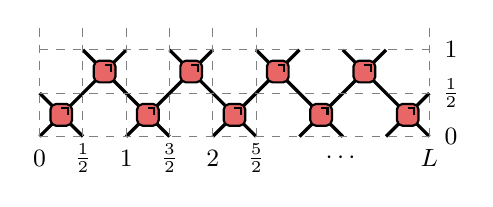
\begin{tikzpicture}[baseline=(current  bounding  box.center), scale=0.55]
\foreach \i in {0,...,4}
{
\Wgatered{2*\i}{-3+0.5};
}
\foreach \i in {0,...,3}
{
\Wgatered{2*\i+1}{-1-0.5}
}
\foreach \i in {0,1,2}
{
\Text[x=2*\i-0.5,y=-3.5]{\small$\i$};
}
\foreach \i in {1,3,5}
{
\Text[x=\i-0.5,y=-3.5]{\small$\frac{\i}{2}$}
}
\Text[x=8.5,y=-3.5]{\small$L$};
\Text[x=6.5,y=-3.5]{\small$\cdots$};
\foreach \j in {0,1}
{
\Text[x=9,y=2*\j-3]{\small$\j$}
}
\foreach \j in {1}
{
\Text[x=9,y=\j-3]{\small$\frac{\j}{2}$}
}
\foreach \i in {0,1,2,3,4,5,9}
{
\draw[gray, dashed] (\i-0.5,-0.5) -- (\i-0.5,-3);
}
\foreach \j in {0,1,2}
{
\draw[gray, dashed] (-0.5,\j-3) -- (8.5,\j-3);
}
\end{tikzpicture}
\end{aligned}
,
\end{equation*}
where $\mathbb{T}_{2L}$ is a periodic translation operator on $2L$ sites, and $u$ a local gate. Here, for simplicity, we assume translational invariance of the circuit and introduce periodic boundary conditions. However, our result can be easily generalized to non-uniform cases and open boundary conditions.
Above, we graphically represented local unitary gates with dimension
$D^{2}\times D^{2}$ by a box with incoming and outgoing legs, \begin{equation}
u=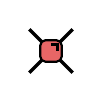
\begin{tikzpicture}[baseline=(current  bounding  box.center), scale=0.55]
\Wgatered{0}{0}
\end{tikzpicture}
,
\qquad
\qquad
u^{\dagger}=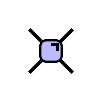
\begin{tikzpicture}[baseline=(current  bounding  box.center), scale=0.55]
\Wgateblue{5}{5}
\end{tikzpicture},
\end{equation}
satisfying unitarity conditions
\begin{equation}\label{eq:unitarity}
\begin{aligned}
&uu^{\dagger}=
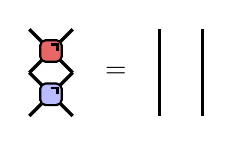
\begin{tikzpicture}[baseline=(current  bounding  box.center), scale=0.55]
\Wgatered{0}{0}
\Wgateblue{0}{-1}
\Text[x=1.5,y=-0.5]{$=$}
\draw[very thick] (2.5,0.5)--(2.5,-1.5);
\draw[very thick] (3.5,0.5)--(3.5,-1.5);
\end{tikzpicture}
=I_{D^2},\\
&u^{\dagger}u=
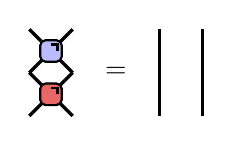
\begin{tikzpicture}[baseline=(current  bounding  box.center), scale=0.55]
\Wgateblue{0}{0}
\Wgatered{0}{-1}
\Text[x=1.5,y=-0.5]{$=$}
\draw[very thick] (2.5,0.5)--(2.5,-1.5);
\draw[very thick] (3.5,0.5)--(3.5,-1.5);
\end{tikzpicture}
=
I_{D^2}.
\end{aligned}
\end{equation}


Our results can be more succinctly expressed in the folded picture, where an operator over $(C^D)^{2L}$ is vectorized to a vector in $(C^D)^{4L}$ by the linear map on the basis
\begin{equation}
\ket{m}\bra{n}\to\ket{m}\ket{n}.
\end{equation}
The time evolution in Schrodinger picture can also be vectorized to
\begin{equation}
u()u^{\dagger}\to u\otimes u^*.
\end{equation}
Graphically, $u^{\dagger}$
is folded back behind $u$, thereby forming a joint operator $w 	\equiv u\otimes u^{*}$.
It is also convenient to denote the vectorized identity operator in the folded picture as an empty bullet $\ket{\mcirc}=\frac{1}{\sqrt{D}}\ket{I_D}$, which is shown below %\pk{We may label the folded gate w if we need it?}
\begin{equation}
w=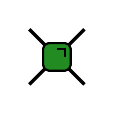
\begin{tikzpicture}[baseline=(current  bounding  box.center), scale=0.7]
\Wgategreen{0}{0}
\end{tikzpicture}
=
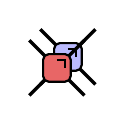
\begin{tikzpicture}[baseline=(current  bounding  box.center), scale=0.7]
\Wgateblue{0.1}{0.1}
\Wgatered{-0.1}{-0.1}
\end{tikzpicture}
,
\qquad
\qquad

\begin{tikzpicture}[baseline=(current  bounding  box.center), scale=0.7]
\MYcircle{0.25}{0.25}
\draw[very thick] (-0.25,-0.25)--(0.20,0.20);
\end{tikzpicture}
=\frac{1}{\sqrt{D}}

\begin{tikzpicture}[baseline=(current  bounding  box.center), scale=0.7]
\draw[very thick] (-0.25,-0.25)--(0.25,0.25)--(0.05,0.45)--(-0.45,-0.05);
\end{tikzpicture}
.
\end{equation} 
With these notations, the unitarity condition~\eqref{eq:unitarity} is graphically expressed as $
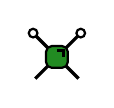
\begin{tikzpicture}[baseline=(current  bounding  box.center), scale=0.55]
\Wgategreen{0}{0}
\MYcircle{0.55}{0.55}
\MYcircle{-0.55}{0.55}
\end{tikzpicture}
=
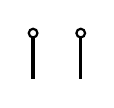
\begin{tikzpicture}[baseline=(current  bounding  box.center), scale=0.55]
\draw[very thick] (-0.55,-0.5) -- (-0.55,0.5);
\draw[very thick] (0.55,-0.5) -- (0.55,0.5);
\MYcircle{0.55}{0.55}
\MYcircle{-0.55}{0.55}
\end{tikzpicture}
$ and $
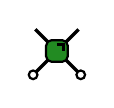
\begin{tikzpicture}[baseline=(current  bounding  box.center), scale=0.55]
\Wgategreen{0}{0}
\MYcircle{0.55}{-0.55}
\MYcircle{-0.55}{-0.55}
\end{tikzpicture}
=
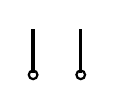
\begin{tikzpicture}[baseline=(current  bounding  box.center), scale=0.55]
\MYcircle{0.55}{-0.55}
\MYcircle{-0.55}{-0.55}
\draw[very thick] (-0.55,-0.5) -- (-0.55,0.5);
\draw[very thick] (0.55,-0.5) -- (0.55,0.5);
\end{tikzpicture}
$.


\subsection{Dual Unitarity}\label{sec:DU}

Understanding the dynamics of extended locally interacting systems is at the core of quantum many-body physics. However, this problem is usually analytically intractable and numerically exponentially hard. 
To make progress, we need some additional structure. One possibility is to demand the so-called dual-unitarity condition~\cite{bertini2019exact} mentioned in the introduction, which enables various exact calculations even for chaotic dynamics.

Dual unitarity demands that the gate $u$ is unitary even if we exchange the roles of space and time. This switching corresponds to changing which are input and output legs of the gate, resulting in the dual local gate $\tilde{u}$.
It is formally introduced by reshuffling the
indices
\be
\label{eq:tildeqgate}
\tilde{u}=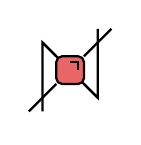
\begin{tikzpicture}[baseline=(current  bounding  box.center), scale=.7]
\draw[ thick] (-4.25,0.5) -- (-3.25,-0.5);
%\draw[ thick] (-4.75,0.5)-- (-4.75,-0.5)--(-4.25,-0.5) -- (-3.25,0.5)-- (-2.75,0.5) -- (-2.75, -0.5);
\draw[thick] (-4,-0.25)--(-4.5,-0.75);
\draw[thick] (-4,0.25)--(-4.25,0.5)--(-4.25,-0.75);
\draw[thick] (-3.5,0.25)--(-3,0.75);
\draw[thick] (-3.5,-0.25)--(-3.25,-0.5)--(-3.25,0.75);
\draw[ thick, fill=myred, rounded corners=2pt] (-4,0.25) rectangle (-3.5,-0.25);
\draw[thick] (-3.75,0.15) -- (-3.75+0.15,0.15) -- (-3.75+0.15,0);
\Text[x=-4.25,y=-0.75]{}
\end{tikzpicture}\;, \, \,
%
\bra{j}\bra{l}\tilde{u}\ket{i}\ket{k}=\bra{k}\bra{l}u\ket{i}\ket{j}.
\ee
A gate is dual-unitary~\cite{bertini2019exact} if both $u$ and $\tilde{u}$ are unitary, so in addition to ~\eqref{eq:unitarity} we also require 
\begin{equation}
\tilde{u}^{\dagger}\tilde{u}=\tilde{u}\tilde{u}^{\dagger}=I_{D^{2}}\label{eq:algebric_dual_unitary},
\end{equation}
which in the folded graphical language yields
\begin{equation}
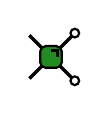
\begin{tikzpicture}[baseline=(current  bounding  box.center), scale=0.55]
\Wgategreen{0}{0}
\MYcircle{0.55}{0.55}
\MYcircle{0.55}{-0.55}
\end{tikzpicture}
=
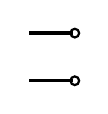
\begin{tikzpicture}[baseline=(current  bounding  box.center), scale=0.55]
\MYcircle{0.55}{0.55}
\MYcircle{0.55}{-0.55}
\draw[very thick] (-0.5,0.55) -- (0.5,0.55);
\draw[very thick] (-0.5,-0.55) -- (0.5,-0.55);
\end{tikzpicture}
,
\qquad
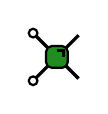
\begin{tikzpicture}[baseline=(current  bounding  box.center), scale=0.55]
\Wgategreen{0}{0}
\MYcircle{-0.55}{0.55}
\MYcircle{-0.55}{-0.55}
\end{tikzpicture}
=
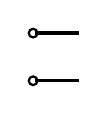
\begin{tikzpicture}[baseline=(current  bounding  box.center), scale=0.55]
\MYcircle{-0.55}{0.55}
\MYcircle{-0.55}{-0.55}
\draw[very thick] (-0.5,0.55) -- (0.5,0.55);
\draw[very thick] (-0.5,-0.55) -- (0.5,-0.55);
\end{tikzpicture}
. \label{eq:figure_dual_unitary_condi}
\end{equation}

The family of models defined in this way encompasses free, interacting integrable and chaotic models~\cite{bertini2019exact}. The parametrization of dual-unitary gates for $D=2$
has been fully determined~\cite{bertini2019exact}.
Despite a lack of the complete parametrization of dual-unitary gates for $D\geq3$, several families have been proposed~\cite{rather2020creating, gutkin2020exact, claeys2021ergodic, aravinda2021from,prosen2021manybody, marton2022construction}. 
We proceed to add another family to the list%suggest a novel parametrization for the $2-$qudit gates
, resulting in a novel extensive family of dual-unitary gates in higher dimensions. This parametrization
also proves useful when addressing the hierarchical generalization
of dual-unitary circuits in the following sections.

Consider the following parametrized family of two-qudit unitary gates:
\begin{equation}
u=(v_{1}\otimes v_{2}) \ u_0 \ (v_{3}\otimes v_{4}),
\label{eq:2quditUgeneralform}
\end{equation}
where $v_{1},v_{2},v_{3},v_{4}$ are single site unitary gates, and $u_0$ is defined as
\begin{equation}
u_0=\sum_{0\leq p,q\leq D-1} \theta_{p,q}\ket{\psi_{p,q}}\bra{\psi_{p,q}}.
\label{eq:CliffordParametrization}
\end{equation}
Here $\{\theta_{p,q}\}_{0\leq p,q\leq D-1}$ is a collection of $\mathrm{U}(1)$ phases, and $\{\ket{\psi_{p,q}}\}_{0\leq p,q\leq D-1}$ is an orthonormal basis for the 2-qudit Hilbert space $(\mathbb{C}^D)^2$ defined as
\begin{equation}
\ket{\psi_{p,q}}\equiv \frac{1}{\sqrt{D}}\sum_{1\leq i,j\leq D}(\tau^p\sigma^q)^*_{ij}\ket{i}\otimes\ket{j},
\label{eq:psi_pq}
\end{equation}
where $\sigma,\tau$ are the $D\times D$ dimensional generators of the Clifford group satisfying the relations
%where $\sigma,\tau$ are constant $D\times D$ matrices satisfying the relations
\begin{equation}\label{eq:ZnCliffordCR}
    \sigma^D=\tau^D=1,~~~ \sigma\tau=\omega\tau\sigma,
\end{equation}
with $\omega=e^{2\pi i/D}$ a $D$-th root of unity. The matrices $\sigma,\tau$ generate the full matrix algebra $M_D(\mathbb{C})$, and we can always choose $\sigma$ to be diagonal and $\tau$ to be real. Explicitly, they are defined as 
\begin{eqnarray}\label{eq:def_sigmatau}
    \sigma&=&\sum^{D-1}_{j=0}\omega^{j}\ket{j}\bra{j},\nonumber\\
    \tau&=&\sum^{D-1}_{j=0}\ket{j+1}\bra{j},\label{eq:definition_of_Clifford}
\end{eqnarray}
where $\ket{D}\equiv \ket{0}$.

We proceed to investigate conditions on the parameters $\{\theta_{p,q}\}_{0\leq p,q\leq D-1}$ for $u$ to be a dual-unitary gate. After a space-time reshuffling of indices defined in Eq.~\eqref{eq:tildeqgate}, we have $\tilde{u}= (v_4^T\otimes v_2)\tilde{u}_0(v_3\otimes v_1^T)$, where
\begin{equation}
    \tilde{u}_0=\frac{1}{D}\sum_{0\leq p,q\leq D-1} \theta_{p,q}\tau_{p,q}\otimes\tau^*_{p,q},
\end{equation}
with $\tau_{p,q}\equiv\tau^p\sigma^q$. Then the unitarity condition~\eqref{eq:algebric_dual_unitary} on $\tilde{u}$ is equivalent to 
\begin{equation}\label{eq:simplifyunitarityClifford}
    \sum_{0\leq p,q,r,s\leq D-1} \theta^*_{p,q}\theta_{r,s}\tau^\dagger_{p,q}\tau_{r,s}\otimes\tau^T_{p,q}\tau^*_{r,s}=D^2 \tau_{0,0}\otimes\tau_{0,0}.
\end{equation}
Notice that the single site unitary gates $v_{1},v_{2},v_{3},v_{4}$ do not appear in the above expression. We simplify Eq.~\eqref{eq:simplifyunitarityClifford} further with the following relations satisfied by $\tau_{p,q}$
\begin{eqnarray}\label{eq:relations_tau_pq}
    \tau_{p,q}\tau_{r,s}&=&\omega^{qr}\tau_{p+r,q+s},\nonumber\\
    \tau^*_{p,q}&=&\tau_{p,-q}\nonumber\\
    \tau^T_{p,q}&=&\omega^{-pq}\tau_{-p,q}.
\end{eqnarray}
They follow from Eqs.~\eqref{eq:ZnCliffordCR} and~\eqref{eq:def_sigmatau} by straightforward computation. Simplifying Eq.~\eqref{eq:simplifyunitarityClifford} using Eq.~\eqref{eq:relations_tau_pq}, and comparing the coefficients of both sides using the fact that $\{\tau_{p,q}\}_{0\leq p,q\leq D-1}$ forms a basis of the matrix algebra $M_D(\mathbb{C})$, we obtain 
\begin{equation}\label{eq:DUcondition_theta}
    \sum_{0\leq p,q\leq D-1} \theta_{p,q}^* \theta_{p+k,q+l} =0,\text{ for }(k,l)\neq (0,0).
\end{equation}
In this way, the original dual unitarity condition, which involves $2D^4$ equations and $2D^4-1$ real unknowns simplifies to a set of $D^2-1$ equations with $D^2-1$ real unknowns~(notice that we can set $\theta_{0,0}=1$ without loss of generality).  A simple yet nontrivial ansatz for $\theta_{p,q}$ is~\footnote{A particularly simple solution to Eq.~\eqref{eq:DUcondition_theta} is
$\theta_{p,q}=\theta_{p+q}\omega^{p^2+pq}$,
where $\{\theta_{p}\}_{p=0}^{D-1}$ are arbitrary U$(1)$ phases. However, this family of dual-unitary gates are actually the same as those given in Eq.~(25) of Ref.~\cite{marton2022construction}.}
\begin{equation}\label{eq:omega_quadratic}
    \theta_{p,q}=\omega^{\lambda p^2+\mu pq+\nu q^2},
\end{equation}
where $\mu\in\mathbb{Z}$, and $\lambda,\nu\in\mathbb{Z}$ if $D$ is odd while $\lambda,\nu\in\mathbb{Z}/2$ if $D$ is even~(which guarantees that $\theta_{p,q}$ is periodic both in $p$ and $q$ with period $D$). Inserting the ansatz~\eqref{eq:omega_quadratic} into Eq.~\eqref{eq:DUcondition_theta}, we see that dual-unitarity requires that $k=l=0$ is the only solution to the following system of equations~\footnote{A sufficient condition for this is that the determinant $4\lambda\nu-\mu^2$ is invertible modulo $D$. }
\begin{eqnarray}
    2\lambda k+\mu l&=&0~(\mathrm{mod}~D),\nonumber\\
    \mu k+2\nu l&=&0~(\mathrm{mod}~D).
\end{eqnarray}
For example, when $D=3$, $\lambda=\mu=1,\nu=-1$ satisfies this condition. In later sections we will use the ansatz Eq.~\eqref{eq:CliffordParametrization} and Eq.~\eqref{eq:omega_quadratic} to find examples of hierarchical generalizations of dual-unitary gates. 

%\pk{Need to discuss the connection with the known extensions of dual-unitarity!}
In this subsection we recapped the basics of dual-unitarity and introduced a novel family of dual-unitary models for $D>2$. A particular subset of solutions from this family appeared before in~\cite{marton2022construction}. This leaves us in a good position to introduce the generalization in the next subsection.

\subsection{Hierarchical Generalization}\label{sec:HG}

As mentioned in the Introduction, dual unitarity imposes conditions on only a single gate, which restricts the possible physical behaviours. It also excludes certain fundamental and well-known gates, such as the Identity and the Controlled-Not gate which are solvable yet not dual-unitary. 
To unveil more intricated quantum dynamics and include these Clifford gates in a more general notion of solvability,
 we define a \emph{hierarchy of conditions}. This gives us new families of  models.
 
 %dual gates  ``Hierarchical gate''. 

Since only one green box plays a part in the dual-unitary condition
(\ref{eq:figure_dual_unitary_condi}), we will call dual-unitarity  also the \emph{first level of the Hierarchy} and denote it as $\mathfrak{L}_1$.
In the subsequent subsections \ref{subsec:Second-Hierarchy}
and \ref{subsec:Third-Hierarchy}, we extend the concept of dual unitarity
($\mathfrak{L}_1$) to conditions involving two and three gates, resulting in the second level $\mathfrak{L}_2$ and
the third level $\mathfrak{L}_3$ of the Hierarchy. %further delving into their parametrizations.

\subsection{Second level of the Hierarchy\label{subsec:Second-Hierarchy}}

In this subsection, we introduce the gates from $\mathfrak{L}_2$, which are more general than dual-unitary gates. $\mathfrak{L}_2$ contains CNOT and identity, as well as a large family of non-trivial gates whose dynamics cannot be solved by any previous techniques and reveals richer physics. The gates from this family fulfill a condition involving two gates, which is weaker than dual-unitary condition:
\begin{equation}
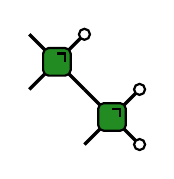
\begin{tikzpicture}[baseline=(current  bounding  box.center), scale=0.7]
\Wgategreen{-0.5}{0.5}
\Wgategreen{0.5}{-0.5}
\MYcircle{0}{1}
\MYcircle{1}{0}
\MYcircle{1}{-1}
\end{tikzpicture}
=
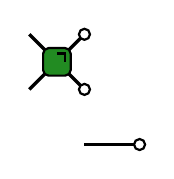
\begin{tikzpicture}[baseline=(current  bounding  box.center), scale=0.7]
\draw[thick] (0,-1)--(1,-1);
\Wgategreen{-0.5}{0.5}
\MYcircle{0}{1}
\MYcircle{0}{00}
\MYcircle{1}{-1}
\end{tikzpicture}
,
\qquad
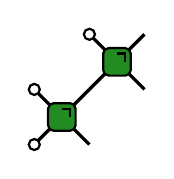
\begin{tikzpicture}[baseline=(current  bounding  box.center), scale=0.7]
\Wgategreen{0.5}{0.5}
\Wgategreen{-0.5}{-0.5}
\MYcircle{0}{1}
\MYcircle{-1}{0}
\MYcircle{-1}{-1}
\end{tikzpicture}
=
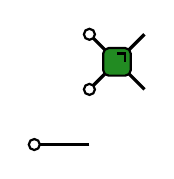
\begin{tikzpicture}[baseline=(current  bounding  box.center), scale=0.7]
\draw[thick] (0,-1)--(-1,-1);
\Wgategreen{0.5}{0.5}
\MYcircle{0}{1}
\MYcircle{0}{0}
\MYcircle{-1}{-1}
\end{tikzpicture}
.\label{eq2:bottomtotop}
\end{equation}
%Since this condition pertains two green boxes situating on the left side, we call it as the $2_{\mathrm{nd}}$ Hierarchical. 
Algebraically, we can express the condition as 
\begin{equation}
\begin{aligned}(I_{D}\otimes\tilde{u}^{\dagger})\cdot\tilde{u}^{\dagger}\tilde{u}\otimes I_{D}\cdot(I_{D}\otimes\tilde{u})=I_{D}\otimes\tilde{u}^{\dagger}\tilde{u},\\
(I_{D}\otimes\tilde{u})\cdot\tilde{u}\tilde{u}^{\dagger}\otimes I_{D}\cdot(I_{D}\otimes\tilde{u}^{\dagger})=I_{D}\otimes\tilde{u}\tilde{u}^{\dagger}.
\end{aligned}
\label{eq:2ndEq}
\end{equation}
A direct observation shows that if a circuit is $\mathfrak{L}_1$, it must be $\mathfrak{L}_2$. This, together with the fact that the identity is in $\mathfrak{L}_2$ but not in $\mathfrak{L}_1$, implies that $\mathfrak{L}_1$ is a proper subset of $\mathfrak{L}_2 \ $:
$\mathfrak{L}_1\subsetneqq\mathfrak{L}_2$. Next we focus on the gates that are in $\mathfrak{L}_2$ but not in $\mathfrak{L}_1$, the set we denote as $\overline{\mathfrak{L}}_2=\mathfrak{L}_2-\mathfrak{L}_1$.


Similarly to the $\mathfrak{L}_1$ case~\cite{bertini2019exact},
we will derive the complete parametrization of the $\overline{\mathfrak{L}}_2$ for the qubits. When $D=2$,
%Eqs. (\ref{eq:2quditUgeneralform}) and (\ref{eq:CliffordParametrization}) are a comprehensive parametrization of all interacting 2-qubit gate and it is more conventional to express $u$ as
an exhaustive parametrization of 2-qubit gates is
\begin{equation}
u=v_{1}\otimes v_{2} \ e^{i(J_{x}\sigma_{x}\sigma_{x}+J_{y}\sigma_{y}\sigma_{y}+J_{z}\sigma_{z}\sigma_{z})} \ v_{3}\otimes v_{4}.
\label{eq:parameter2qubit}\end{equation}
Here $\sigma_i$ are Pauli matrices and $v_{1},v_{2},v_{3},v_{4}$ are all single site
gates from $\mathbb{SU}(2)$. We may simplify the gate structure by setting $v_{3}=v_{4}=I_{D}$
without any loss of generality~\footnote{This is true because because $v_{1}$ at this time step can be
combined with $v_{4}$ from the next time step, allowing for the redefinition
$v_{1}\to v_{4}\cdot v_{1}$. This reasoning also applies to $v_{2}$ and $v_{3}$.}.
%
The trivial example from $\overline{\mathfrak{L}}_2$ is a tensor product of two single-site operators.
Apart from that, the $\overline{\mathfrak{L}}_2$ 
condition fixes $J_{z}=\frac{\pi}{4},J_{x}=J_{y}=0$~\footnote{The permutations among $x,y,z$ also work.} and $v_{1},v_{2}$ to be elements of the set 

\begin{equation}
\{U(r,\theta,\phi)|\sqrt{2}\sin r\sin\theta=\pm1\}, 
\label{eq:condition2ndqubit}
\end{equation}
where $U(r,\theta,\phi)$ is defined as $e^{ir(\cos\theta \ \sigma_{z}+\sin\theta\ \cos\phi \ \sigma_{x}+\sin\theta \ \sin\phi \ \sigma_{y})}$, 
representing a $\mathbb{SU}(2)$ on the Bloch sphere. Geometrically,
this specific combination of $r,\theta,\phi$ represents a rotation that
maps $\sigma_{z}$ to the $x-y$ plane.


The dimension of $\overline{\mathfrak{L}}_2$ can be counted as follows. Out of $12$ parameters determining the $4$ local $\mathbb{SU}(2)$ gates, e.g. the Euler angles, two are redundant because the rotation around the $z-$axis commutes with the Ising interaction resulting from $J_z=\frac{\pi}{4},J_x=J_y=0$. Further, Eq. (\ref{eq:condition2ndqubit}) provides $2$ constraints. After considering the global phase, the total independent parameters to characterize a qubit $\overline{\mathfrak{L}}_2$ circuit is $12-2-2+1$. Therefore, we have defined a new $9$-dimensional %~\footnote{It is 4 dimensional after setting the gauge freedom $v_3=v_4=I_D$.} 
family of solvable models which are not part of $12$-dimensional set of $\mathfrak{L}_1$ gates~\cite{prosen2021manybody}.
%The counting deduces from $16$ parameters two because $\sigma_Z$ commutes and two from the two equations ... and three since $J_i$ are fixed, whereas in $1^\mathrm{st}$ Hierarchical we have $16-2-2=12$ (two $J_i$ fixed and two from commuting $\sigma-Z$).





Note that the control not gate ($\mathrm{CNOT}$) can be decomposed into the form of Eq. (\ref{eq:parameter2qubit}) as 
\begin{equation}
\begin{aligned}
v_1 & =e^{-i\frac{\pi}{4}\sigma_{z}},\; & v_2 & = H\sigma_{x}\cdot e^{i\frac{\pi}{4}\sigma_{z}},\\
v_3 & =I_2,\; & v_4 & =\sigma_{x}H.
\end{aligned}
%\end{aligned}
%\mathrm{CNOT}=(e^{-i\frac{\pi}{4}\sigma_{z}}\otimes H\sigma_{x}\cdot e^{i\frac{\pi}{4}\sigma_{z}})e^{i\frac{\pi}{4}\sigma_{z}\sigma_{z}}\cdot(I_{2}\otimes\sigma_{x}H)e^{-i\frac{\pi}{4}}
\end{equation}
with $J_x=0,J_y=0,J_z=\frac{\pi}{4}$ and an addition global phase $e^{-i\frac{\pi}{4}}$.
H=$\frac{1}{\sqrt{2}}\begin{pmatrix}1 & 1\\
1 & -1
\end{pmatrix}$ is the Hadamard gate, 
and $v_{4}$ can be absorbed into $v_{1}$. It is easy to check that the single site operator gate $v_{1}$ and $v_{2}$ satisfy~\eqref{eq:condition2ndqubit}.
%generate the desired rotation for $\sigma_{z}$, thus a $2^\mathrm{nd}$ Hierarchical.




In higher dimensions, we do not yet possess a complete parametrization
for the $\mathfrak{L}_2$ case. Nevertheless, we can discern two
distinct and rich families. The first family is associated with generalized
Controlled-NOT gate in higher dimension surrounded by $4$ single site operators
\begin{equation}
u=v_1 \otimes v_2 \ \ C_{\tau} \ \ v_3 \otimes v_4,
\end{equation}
with 
$C_{\tau}=\sum_{i}\ket{i}\bra{i}\otimes \tau^{i}$.
%Here $\tau$ is the generator of the Clifford group defined in Eq. (\ref{eq:definition_of_Clifford}). 
Following a similar argument as below Eq. (\ref{eq:parameter2qubit}), we set $v_3=v_4=I_D$. In this case, $v_{1}$ and $v_{2}$
must satisfy
\begin{equation}
\begin{aligned}\sum_{j}\bra{j}v_{1}\ket{i}\bra{j+k'-k}v_{1}^{*}\ket{i} & =\delta_{k,k'}\ \mathrm{for}\ \forall k,k',i.\\
\sum_{j}\bra{i}v_{2}\ket{j}\bra{i}v_{2}^{*}\ket{j+k'-k} & =\delta_{k,k'}\ \mathrm{for}\ \forall k,k',i.
\end{aligned}
\end{equation}
These two equations share a symmetry of exchanging columns and rows between themselves. 


The second family is derived using the Clifford group method from subsection~\ref{sec:DU}. Utilizing the proposed ansatz from Eqs. (\ref{eq:2quditUgeneralform}) and (\ref{eq:CliffordParametrization}), we set $v_3=v_4=I_D$ and simplify Eq. (\ref{eq:2ndEq}) to: 
\begin{widetext}
\begin{equation}
\begin{aligned}(\sum_{b}\theta_{p_{b},q_{b}}^{*}\theta_{p_{b}+k,q_{b}+l})(\sum_{d}\theta_{p_{d},q_{d}}^{*}\theta_{p_{d}+s,q_{d}+t}\tau_{p_{d},q_{d}}^{\dagger}v_{1}^{*}\tau_{k,-l}v_{1}^{T}\tau_{p_{d},q_{d}})=0,\ \\
(\sum_{b}\theta_{p_{b},q_{b}}^{*}\theta_{p_{b}+k,q_{b}+l})(\sum_{d}\theta_{p_{d},q_{d}}^{*}\theta_{p_{d}+s,q_{d}+t}\tau_{-p_{d},q_{d}}^{\dagger}v_{2}^{*}\tau_{-k,-l}v_{2}^{T}\tau_{-p_{d},q_{d}})=0.
\end{aligned}\label{eq:Clifford_parametrization_2nd_result}
\end{equation}
\end{widetext}
Here $\sum_b$ is a shorthand for $\sum_{0\leq p_b,q_b\leq D-1}$. %, the same for $\sum_d$ 
The above equation should hold for $\forall(s,t)\neq(0,0)\ \mathrm{and}\ (k,l)\neq(0,0)$. If all terms in the first sum vanish separately, we obtain the $\mathfrak{L}_1$. 
From these nonlinear equations, we can derive a family of $\overline{\mathfrak{L}}_2$, which is just one of the many possible solutions.
The family is defined for $ D=4k+2$ as
\begin{equation}
 %  v_{i}=I_{D}, \; \,  
 k\in\mathbb{N}^{+}\, \; \mathrm{ and }\,\; \theta_{p,q}=\omega^{\frac{Dpq}{2}} \, .
    \label{eq:simplest_2nd_Hierarchy_case}
\end{equation}
Another nontrivial example is given by 
\begin{equation}
\theta_{p,q}=\begin{cases}
\omega^{\frac{p^{2}}{2}} & D=\mathrm{even}\\
\omega^{p^{2}} & D=\mathrm{odd}
\end{cases}\; ,\end{equation}
%which is also a valid $\overline{\mathfrak{L}}_2$ Hierarchical circuit, 
%this time with some nontrivial $v_{1}$ and $v_{2}$.
In both of the two examples, the so far unspecified $v_1$ and $v_2$ belong a non-trivial subset of $\mathbb{SU}(D)$. These subsets can be deduced from the second sums of Eq.~\eqref{eq:Clifford_parametrization_2nd_result}. Different choices lead to both ergodic and non-ergodic dynamic.


Before concluding this subsection, we would like to highlight that Eq. (\ref{eq2:bottomtotop})
additionally implies

\begin{equation}
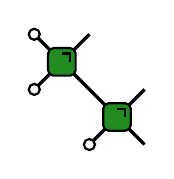
\begin{tikzpicture}[baseline=(current  bounding  box.center), scale=0.7]
\Wgategreen{-0.5}{0.5}
\Wgategreen{0.5}{-0.5}
\MYcircle{-1}{1}
\MYcircle{-1}{0}
\MYcircle{0}{-1}
\end{tikzpicture}
=
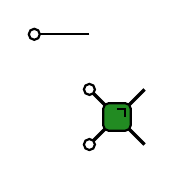
\begin{tikzpicture}[baseline=(current  bounding  box.center), scale=0.7]
\Wgategreen{0.5}{-0.5}
\draw[thick] (0,1)--(-1,1);
\MYcircle{-1}{1}
\MYcircle{0}{0}
\MYcircle{0}{-1}
\end{tikzpicture}
,
\qquad
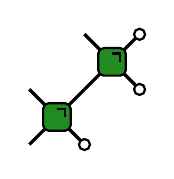
\begin{tikzpicture}[baseline=(current  bounding  box.center), scale=0.7]
\Wgategreen{-0.5}{-0.5}
\Wgategreen{0.5}{0.5}
\MYcircle{1}{1}
\MYcircle{1}{0}
\MYcircle{0}{-1}
\end{tikzpicture}
=
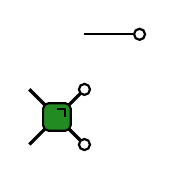
\begin{tikzpicture}[baseline=(current  bounding  box.center), scale=0.7]
\Wgategreen{-0.5}{-0.5}
\draw[thick] (0,1)--(1,1);
\MYcircle{1}{1}
\MYcircle{0}{0}
\MYcircle{0}{-1}
\end{tikzpicture}
.
\label{eq:2ndfig}
\end{equation}
The proof is shown in Appendix \ref{app:proof2nd}. 
 Eq. (\ref{eq:2ndfig}) will play an important role in computing the spatio-temporary correlation functions.


\subsection{Third level of the Hierarchy\label{subsec:Third-Hierarchy}}

Following the principles from subsection \ref{subsec:Second-Hierarchy}, we define the third level hierarchical condition for $\mathfrak{L}_3$ as 
\begin{equation}
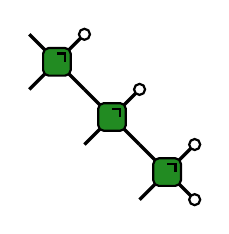
\begin{tikzpicture}[baseline=(current  bounding  box.center), scale=0.7]
\Wgategreen{-1.5}{0.5}
\Wgategreen{-0.5}{-0.5}
\Wgategreen{-2.5}{1.5}
\MYcircle{-1}{1}
\MYcircle{0}{0}
\MYcircle{0}{-1}
\MYcircle{-2}{2}
\end{tikzpicture}
=
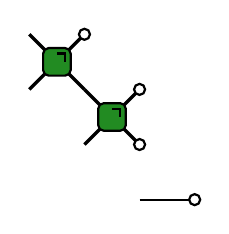
\begin{tikzpicture}[baseline=(current  bounding  box.center), scale=0.7]
\Wgategreen{-1.5}{0.5}
\Wgategreen{-2.5}{1.5}
\draw[thick] (-1,-1)--(0,-1);
\MYcircle{0}{-1}
\MYcircle{-1}{0}
\MYcircle{-1}{1}
\MYcircle{-2}{2}
\end{tikzpicture}
.\label{eq:3rdHierarchydefinition}
\end{equation}An immediate observation reveals that a gate characterized as $\mathfrak{L}_2$ is also the $\mathfrak{L}_3$. Nonetheless, we are again interested
in the special subset of $\mathfrak{L}_3$ which does not belong to
$\mathfrak{L}_2$, designated as $\overline{\mathfrak{L}}_3=\mathfrak{L}_3-\mathfrak{L}_2$.
A notable example within $\overline{\mathfrak{L}}_3$ is the controlled-Z gate.

We again use the complete parameterization of 2-qubit gates (\ref{eq:parameter2qubit}) and wlog set $v_3=v_4=I_2$. The condition defining $\overline{\mathfrak{L}}_3$ is satisfied either for all diagonal gates or for the case where $J_{x}=J_{y}=0$ and any $J_z$ with $v_i$ satisfying $v_i=\cos{\phi_i}\sigma_x+\sin{\phi_i}\sigma_y,i\in{1,2}$. %, meaning that they lie on the equator of the Bloch sphere.

To get some examples for $D>2$, we use our Clifford gate parametrization method
from Secion~\ref{sec:DU}. 
The algebraic equation
of $\theta_{p,q}$ can be found in the Appendix~\ref{sec:appendixA}. To obtain some examples, we take the single-site operators $v_i$ to be the identity. Some classes of the solutions obtained in this way are shown below.
\begin{equation}
\theta_{p,q}=\begin{cases}
\omega^{p^{2}+\frac{3}{2}q^{2}} & D=12m+2;\\
\omega^{p^{2}+q^{2}} & D=8m+4;\\
\omega^{p^{2}+\frac{3}{2}q^{2}} & D=12m+6,m\neq1\ \mathrm{mod}\ 3;\\
\omega^{p^{2}+\frac{3}{2}q^{2}} & D=12m+10.
\end{cases}
\end{equation}

In principle, nothing stops us from going beyond the $\mathfrak{L}_3$, by demanding even more general condition with even more gates. We expect the examples to be constructed in a similar way.
%--------------------------------------------------------------
\section{Applications}
\label{sec:applications}
\subsection{Spatio-temporary correlator functions}\label{subsec:STCF}
In this subsection we focus on the spatio-temporal correlation functions, which are the most common objects to characterize the dynamics. In particular, they provide information about the thermalization and ergodicity of the system. %Macroscopically, the two-point correlation function is in the framework of linear response theory to express conductivity and viscosity.

In most cases, the exact non-perturbative calculation of the spatio-temporary correlators is only available in free models and to some extent in interacting integrable ones~\cite{Medenjak_2017,Klobas_2019,Klobas_2021}. 
Important progress has been made in understanding the correlations also in chaotic models, in particular dual-unitary ($\mathfrak{L}_1$) circuits which we extend here.


%sometimes referred to as OTOC\pk{OTOCs are different objects, we can discuss}. 
Due to the trivial propagation of an identity operator, we are only interested in the correlation function between two traceless Hilbert-Schmidt normalized operators $a_{i},b_{j}$\footnote{Hilbert Schmidt normalized means that $\mathrm{Tr}a_i^\dagger a_i=1$}.
Working in the Heisenberg picture, the spatio-temporal correlation function of normalized local operators can be expressed as %\pk{factors of D? Normalization of a,b?}
\begin{equation}
C_{ij}(t)=\langle a_{i}(t)b_{j}\rangle=D\mathrm{Tr}\left((\mathbb{U}^t)^{\dagger} a_{i}\mathbb{U}^tb_{j}\frac{1}{D^{2L}}\right),
\label{eq:definitionofcorrelationfunction}
\end{equation}
%In this subsection, we take the temperature to be infinity, equivalently, the initial state is the maximally mixed state. 
The factor $\frac{1}{D^{2L}}$ comes from the normalized infinite temperature state $\rho_{\infty}=\frac{I_{D^{2L}}}{D^{2L}}$. We also include a prefactor $D$ in the definition to ensure that the autocorrelation function at time $0$ is normalized to $1$. Alternatively, this can be viewed as a quench from the $b_j \1$ state, i.e. $b_j$ applied to the maximally mixed state. 
The correlations in the folded picture are graphically
expressed as %\pk{factors of D?}
\begin{align}
&C_{ij}(t)=
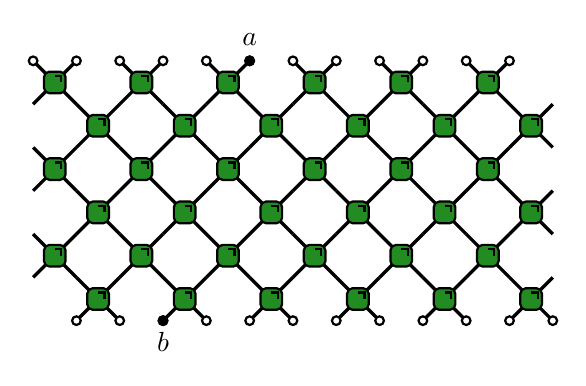
\begin{tikzpicture}[baseline=(current bounding box.center), scale=0.55]
\foreach \jj[evaluate=\jj as \j using -2*(ceil(\jj/2)-\jj/2)] in {0,...,5}
\foreach \i in {1,...,6}
{\Wgategreen{2*\i+\j}{\jj}}
\foreach \i in {2,...,13}{
\MYcircle{\i-.5}{-0.5}
\MYcircle{\i-1.5}{6-0.5}
}
\MYcircleB{3.5}{-.5}
\MYcircleB{5.5}{6-.5}
\Text[x=3.5,y=-1.0]{$b$}
\Text[x=5.5,y=6.0]{$a$}
\end{tikzpicture}\, . \label{eq:Corr1}
\end{align}
Employing the time unitarity enables us to simplify the circuit from the bottom
and top, yielding

\begin{align}
&C_{ij}(t)=
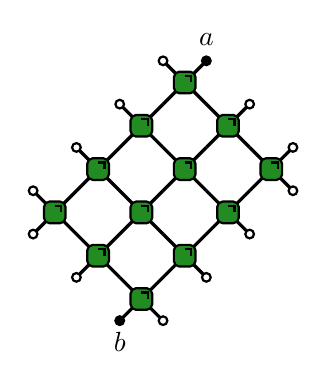
\begin{tikzpicture}[baseline=(current bounding box.center), scale=0.55]
\Wgategreen{3}{0}
\Wgategreen{2}{1}
\Wgategreen{4}{1}
\Wgategreen{1}{2}
\Wgategreen{3}{2}
\Wgategreen{5}{2} 
\Wgategreen{2}{3}
\Wgategreen{4}{3}
\Wgategreen{6}{3}
\Wgategreen{3}{4} 
\Wgategreen{5}{4}
\Wgategreen{4}{5}
\MYcircle{1.5}{0.5}
\MYcircle{0.5}{1.5}
\foreach \i in {1,...,4}
{\MYcircle{2.5+\i}{\i-1.5}}
\foreach \i in {1,...,4}
{
\MYcircle{4.5-\i}{6.5-\i}
}
\MYcircle{5.5}{4.5}
\MYcircle{6.5}{3.5}
\MYcircleB{2.5}{-.5}
\MYcircleB{4.5}{6-.5}
\Text[x=2.5,y=-1.0]{$b$}
\Text[x=4.5,y=6.0]{$a$}
\end{tikzpicture}\, . 
\label{eq:2pointaftertimeuni}
\end{align}

\subsubsection{Dual unitarity}
For completeness, here we briefly summarize the result for dual-unitary circuit from~\cite{bertini2019exact}. 
Intuitively, the time unitarity and space unitarity both determine a light cone outside which the correlation function vanishes. Therefore, correlators can solely manifest at the intersection of these two cones, forming a 1-dimensional straight line that precisely bisects the temporal and spatial directions
\begin{equation}\label{eq:diagonal}
\begin{aligned}
&C_{ij}(t)=
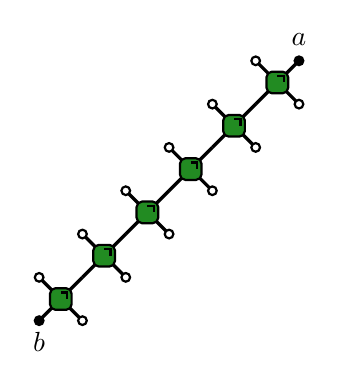
\begin{tikzpicture}[baseline=(current bounding box.center), scale=0.55]
\foreach \i in {0,...,5}
{\Wgategreen{3+\i}{\i}}
\foreach \i in {0,...,5}
{\MYcircle{2.5+\i}{0.5+\i}}
\foreach \i in {0,...,5}
{\MYcircle{3.5+\i}{-0.5+\i}}
\MYcircleB{2.5}{-.5}
\MYcircleB{8.5}{6-.5}
\Text[x=2.5,y=-1.0]{$b$}
\Text[x=8.5,y=6.0]{$a$}
\end{tikzpicture}
,
\end{aligned}
\end{equation}
with other correlators vanishing. That other correlations vanish can be seen by repeatedly applying~\eqref{eq:figure_dual_unitary_condi} to expression~\eqref{eq:2pointaftertimeuni}, which results in $\braket{\mcirc|\mcircf}=0$ since the operators $a$ and $b$ are traceless.
In Eq.~\eqref{eq:diagonal} each time step is just a quantum channel over $D\times D$ Hilbert space. Therefore, the correlators for the $\mathfrak{L}_1$ circuits can always be calculated efficiently and propagates only along two directions with maximal speed.

\subsubsection{$\overline{\mathfrak{L}}_2$ circuits}
Moving beyond the $\mathfrak{L}_1$, we are interested in which new features appear in the $\overline{\mathfrak{L}}_2$ circuits.
Said differently, we are interested in what happens if the weaker condition~\eqref{eq2:bottomtotop} defining $\mathfrak{L}_2$ is satisfied but dual unitarity condition~\eqref{eq:figure_dual_unitary_condi} is not.

We apply Eq. (\ref{eq2:bottomtotop}) to Eq. (\ref{eq:2pointaftertimeuni}) and further simplify the circuit to
\begin{align}
&C_{ij}(t)=
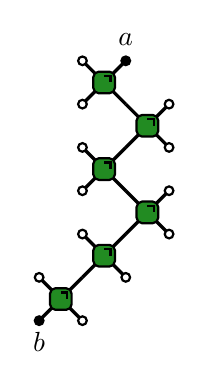
\begin{tikzpicture}[baseline=(current bounding box.center), scale=0.55]
\Wgategreen{4}{5}
\Wgategreen{5}{4}
\Wgategreen{4}{3}
\foreach \i in {1,2,3}
{\Wgategreen{2+\i}{\i-1}}
\foreach \i in {1,...,5}
{
\MYcircle{3.5}{\i+0.5}
}
\foreach \i in {1,2,3}
{\MYcircle{5.5}{1.5+\i}}
\MYcircle{2.5}{0.5}
\foreach \i in {1,2,3}
{\MYcircle{2.5+\i}{\i-1.5}}
\MYcircleB{2.5}{-.5}
\MYcircleB{4.5}{6-.5}
\Text[x=2.5,y=-1.0]{$b$}
\Text[x=4.5,y=6.0]{$a$}
\end{tikzpicture}\, .
\end{align}
Lastly, Eq. (\ref{eq:2ndfig}) is utilised to address the corner of the
path, leading to\begin{align}
&C_{ij}(t)=
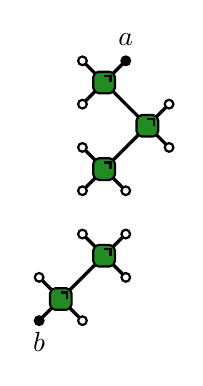
\begin{tikzpicture}[baseline=(current bounding box.center), scale=0.55]
\Wgategreen{4}{5}
\Wgategreen{5}{4}
\Wgategreen{4}{3}
\foreach \i in {1,2}
{\Wgategreen{2+\i}{\i-1}}
\foreach \i in {1,...,5}
{
\MYcircle{3.5}{\i+0.5}
}
\foreach \i in {2,3}
{\MYcircle{5.5}{1.5+\i}}
\MYcircle{2.5}{0.5}
\foreach \i in {1}
{\MYcircle{2.5+\i}{\i-1.5}}
\foreach \i in {1,2,3}
{\MYcircle{4.5}{\i-0.5}}
\MYcircleB{2.5}{-.5}
\MYcircleB{4.5}{6-.5}
\Text[x=2.5,y=-1.0]{$b$}
\Text[x=4.5,y=6.0]{$a$}
\end{tikzpicture}\, .
\end{align}
This correlator vanishes because the discontinuous path will be simplified to $\mathrm{\mathrm{Tr}}a_{i}\mathrm{Tr}b_{j}$ and both are traceless according to our assumption.

Therefore, the existence of nonvanishing correlators is limited to three possible directions, either at the light cone or at velocity zero. %\pk{strictly speaking notation is wrong, RHS is allways non 0}

\begin{equation}
\begin{aligned}
&C_{ij}(t)=
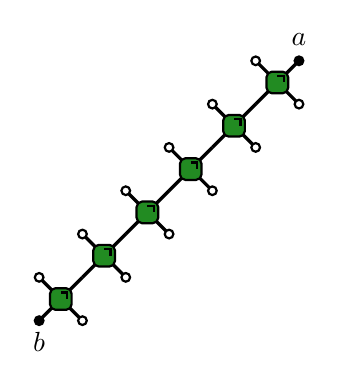
\begin{tikzpicture}[baseline=(current bounding box.center), scale=0.55]
\foreach \i in {0,...,5}
{\Wgategreen{3+\i}{\i}}
\foreach \i in {0,...,5}
{\MYcircle{2.5+\i}{0.5+\i}}
\foreach \i in {0,...,5}
{\MYcircle{3.5+\i}{-0.5+\i}}
\MYcircleB{2.5}{-.5}
\MYcircleB{8.5}{6-.5}
\Text[x=2.5,y=-1.0]{$b$}
\Text[x=8.5,y=6.0]{$a$}
\end{tikzpicture}
,\\
&C_{ij}(t)=
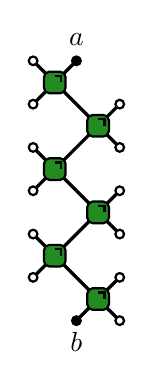
\begin{tikzpicture}[baseline=(current bounding box.center), scale=0.55]
\foreach \i in {0,1,2}
{
\Wgategreen{4}{2*\i}
\Wgategreen{3}{1+2*\i}
\MYcircle{4.5}{2*\i-0.5}
\MYcircle{4.5}{2*\i+0.5}
\MYcircle{2.5}{1.5+2*\i}
\MYcircle{2.5}{0.5+2*\i}
}
\MYcircleB{3.5}{-.5}
\MYcircleB{3.5}{6-.5}
\Text[x=3.5,y=-1.0]{$b$}
\Text[x=3.5,y=6.0]{$a$}
\end{tikzpicture}
.
\end{aligned}
\label{eq:finalresult1site}
\end{equation}
%The aforementioned findings can be articulated in the context of quantum channels.
These expressions can be written using four single qudit channels: 
\begin{equation}
\begin{aligned}
&\epsilon_L(b)=
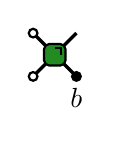
\begin{tikzpicture}[baseline=(current bounding box.center), scale=0.55]
\Wgategreen{0}{0}
\MYcircle{-0.5}{-0.5}
\MYcircle{-0.5}{0.5}
\MYcircleB{0.5}{-0.5}
\Text[x=0.5,y=-1]{$b$}
\end{tikzpicture}
,
\qquad
&\epsilon_R(b)=
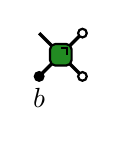
\begin{tikzpicture}[baseline=(current bounding box.center), scale=0.55]
\Wgategreen{0}{0}
\MYcircle{0.5}{-0.5}
\MYcircle{0.5}{0.5}
\MYcircleB{-0.5}{-0.5}
\Text[x=-0.5,y=-1]{$b$}
\end{tikzpicture}
,\\
&M_L(b)=
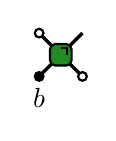
\begin{tikzpicture}[baseline=(current bounding box.center), scale=0.55]
\Wgategreen{0}{0}
\MYcircle{0.5}{-0.5}
\MYcircle{-0.5}{0.5}
\MYcircleB{-0.5}{-0.5}
\Text[x=-0.5,y=-1]{$b$}
\end{tikzpicture}
,
\qquad
&M_R(b)=
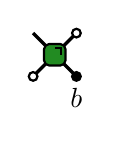
\begin{tikzpicture}[baseline=(current bounding box.center), scale=0.55]
\Wgategreen{0}{0}
\MYcircle{-0.5}{-0.5}
\MYcircle{0.5}{0.5}
\MYcircleB{0.5}{-0.5}
\Text[x=0.5,y=-1]{$b$}
\end{tikzpicture}
.
\end{aligned}
\end{equation}
%These channels enable the expression of correlation functions in a more streamlined manner. 
To simplify the analysis, we assume $j$ to be an integer, and the other case follows analogously. Thus
\begin{equation}
C_{ij}(t)=\begin{cases}
\mathrm{Tr}\left(aM_{L}^{2t}(b)\right) & t=i-j\\
\mathrm{Tr}\left(a(\epsilon_{R})^{k}(\epsilon_{L}\epsilon_{R})^{\lfloor\frac{t}{2}\rfloor}(b)\right) & i=j,t=\mathbb{Z}+\frac{k}{2}\\
0 & \mathrm{otherwise}
\end{cases}\label{eq:expression_CF_1site}
\end{equation}
%\pk{what is kappa in the above eq?} 
This $C_{ij}(t)$ behaves differently than
that in the dual-unitary case~\cite{bertini2019exact}, %, wherein non-zero values only emerge at the light cone. 
as the circuits from $\mathfrak{L}_2$ allow for an additional non-vanishing direction along the time axis. 

Let us mention here the connection with tri-unitaries circuits proposed in \cite{jonay2021triunitary}, where the correlation function also exclusively manifest in the same three directions. In fact, we can group the legs of two 2-qubit gates into a 3-qubit gates as
\begin{equation}
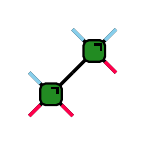
\begin{tikzpicture}[baseline=(current bounding box.center), scale=0.55]
    \Wgategreen{0}{0}
    \Wgategreen{-1}{-1}
    \draw[red!70!magenta,very thick] (-1.25,-1.25)--(-1.5,-1.5);
    \draw[red!70!magenta,very thick] (-0.75,-1.25)--(-0.5,-1.5);
    \draw[red!70!magenta,very thick] (0.25,-0.25)--(0.5,-0.5);
    \draw[skyblue, very thick] (-1.25,-0.75) -- (-1.5,-0.5);
    \draw[skyblue, very thick](-0.25,0.25) -- (-0.5,0.5);
    \draw[skyblue, very thick](0.25,0.25) -- (0.5,0.5);
\end{tikzpicture}
\Rightarrow
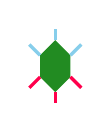
\begin{tikzpicture}[baseline=(current bounding box.center), scale=0.55]
 \fill[mygreen] (0,0) -- (0.35,0.35) -- (0.35,0.85) -- (0,1.2) -- (-0.35,0.85) -- (-0.35,0.35) -- cycle;
 \draw[red!70!magenta,very thick](0,0)--(0,-0.25);
 \draw[red!70!magenta,very thick](0.35,0.35)--(0.6,0.1);
 \draw[red!70!magenta,very thick](-0.35,0.35)--(-0.6,0.1);
 \draw[skyblue, very thick](0,1.2)--(0,1.45);
 \draw[skyblue, very thick](0.35,0.85) -- (0.6,1.1);
 \draw[skyblue, very thick](-0.35,0.85) -- (-0.6,1.1);
\end{tikzpicture}\; .
\end{equation}
However, in the tri-unitary case, the condition is
\begin{equation}
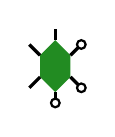
\begin{tikzpicture}[baseline=(current bounding box.center), scale=0.55]
 \fill[mygreen] (0,0) -- (0.35,0.35) -- (0.35,0.85) -- (0,1.2) -- (-0.35,0.85) -- (-0.35,0.35) -- cycle;
 \draw[very thick](0,0)--(0,-0.25);
 \draw[very thick](0.35,0.35)--(0.6,0.1);
 \draw[very thick](-0.35,0.35)--(-0.6,0.1);
 \draw[very thick](0,1.2)--(0,1.45);
 \draw[very thick](0.35,0.85) -- (0.6,1.1);
 \draw[very thick](-0.35,0.85) -- (-0.6,1.1);
 \MYcircle{0.6}{0.1}
 \MYcircle{0}{-0.25}
 \MYcircle{0.6}{1.1}
\end{tikzpicture}
=
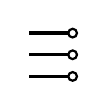
\begin{tikzpicture}[baseline=(current bounding box.center), scale=0.55]

\draw[very thick](-0.5,1)--(0.5,1);
\draw[very thick](-0.5,0.5)--(0.5,0.5);
\draw[very thick](-0.5,0)--(0.5,0);
\MYcircle{0.5}{1}
\MYcircle{0.5}{0.5}
\MYcircle{0.5}{0}
\end{tikzpicture}
\end{equation}
which is a much stronger condition than Eq. (\ref{eq2:bottomtotop}).

Interestingly, in the context of qubits ($D=2$), it is impossible to observe all in principle allowed physical behaviors.
The correlations along the light rays vanish since channels $\epsilon_{L}$ and $\epsilon_{R}$ correspond to the total depolarizing channel.
%Furthermore, %after an extensive algebraic computations \pk{as written not clear what we want to say} it can be explicitly shown that the correlators along the same timeline will vanish exactly after a half step. 
Nevertheless, when $D>2$, there are examples manifesting all of the properties discussed above, i.e. nonvanishing correlations in all three directions at all times. 
In other words, both the correlations in Eq. (\ref{eq:finalresult1site}) are nontrivial. A such example is given in Eq. (\ref{eq:simplest_2nd_Hierarchy_case}) which is also shown in Fig. \ref{Correlation_func_sup2}(a). In this figure, the operator has support on two nearest neighbor sites, to eliminate the odd/even effect (for details see subsec. \ref{subsec:Biggersupports}). 
%\pk{Need to adress Bruno's comment somewhere: Do I understand correctly that for D high enough the second correlation in Eq. 38 becomes non-trivial? Does the transfer matrix have non-trivial eigenvalues or it’s just a large Jordan block?}

\subsubsection{$\overline{\mathfrak{L}}_3$ and higher levels}
In the case where the gate is classified as $\overline{\mathfrak{L}}_3$, the correlation
function is reduced to  %\pk{bullet missing}
\begin{equation}
C_{ij}(t)=
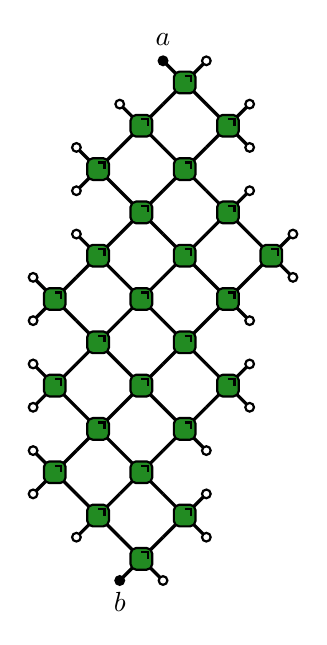
\begin{tikzpicture}[baseline=(current bounding box.center), scale=0.55]
\foreach \i in {0,...,5}
{\Wgategreen{0}{2*\i}}
\foreach \i in {0,...,5}
{
\Wgategreen{1}{1+2*\i}
}
\foreach \i in {0,...,4}
{\Wgategreen{-1}{1+2*\i}}
\foreach \i in {0,...,3}
{\Wgategreen{2}{4+2*\i}}
\foreach \i in {0,1,2}
{
\Wgategreen{-2}{2+2*\i}
}
\Wgategreen{3}{7}
\foreach \i in {0,1,2}
{
\MYcircle{-1.5}{7.5+\i}
\MYcircle{1.5}{0.5+\i}
\MYcircle{2.5}{3.5+\i}
\MYcircle{2.5}{8.5+\i}
}
\foreach \i in {0,...,5}
{
\MYcircle{-2.5}{1.5+\i}
}
\MYcircle{0.5}{-0.5}
\MYcircle{3.5}{6.5}
\MYcircle{3.5}{7.5}
\MYcircle{1.5}{11.5}
\MYcircle{-0.5}{10.5}
\MYcircleB{-0.5}{-0.5}
\MYcircleB{0.5}{11.5}
\MYcircle{-1.5}{0.5}
\Text[x=-0.5,y=-1] {$b$};
\Text[x=.5,y=12] {$a$};
\end{tikzpicture}
.
\end{equation}
Intriguingly, this correlator does not vanish within the entire light cone, and no closed expression for it can be derived with a scaling polynomial in system size. Nevertheless, the hierarchical conditions influences the velocity of the light cone, slowing it down. As a general rule, for a $k$th level of Hierarchical circuit $\mathfrak{L}_k$, the velocity of the light cone will be suppressed to $\nu_k=\frac{k-2}{k}$.


\subsection{Bigger operators and higher orders}
\label{subsec:Biggersupports}

In contrast to previous research, which concentrated primarily on correlators supported on a single site, exploring operators with multi-site support sheds light on more intricate underlying physical phenomena. %Specifically, for correlators supported on two nearest-neighbor sites,
Specifically, for correlators supported on multiple sites, their behavior resembles that described in Eq. (\ref{eq:expression_CF_1site}), where correlation functions manifest exclusively along three directions. Remarkably, in the case of qubits, these correlation functions persist over time unlike the single-site supported ones.

Here we present examples of the correlators on nearest neighbor sites. The derivation is essential the same as in the previous section with some special attention to the simplifications around the operators. The location of a multi-site operator is indexed by its leftmost site. For simplicity, we assume $j$ is an even number and represent the nearest neighbor two-site operator by a black square 
\begin{tikzpicture}[baseline=(current bounding box.center), scale=0.55]
\MYsquareB{4}{0}
\draw[very thick](3.75,0.25)--(3.5,0.5);
\draw[very thick](4.25,0.25)--(4.5,0.5);
\end{tikzpicture} $=$ 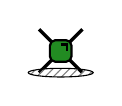
\begin{tikzpicture}[baseline=(current bounding box.center), scale=0.55]
\Wgategreen{0}{0}
\fill[pattern=north east lines, pattern color=gray, postaction={draw=black}] (0,-0.5) ellipse (0.75 and 0.1);
\end{tikzpicture}.
%
%
\begin{equation}
\braket{a_{j+t-1}(t) b_j}=
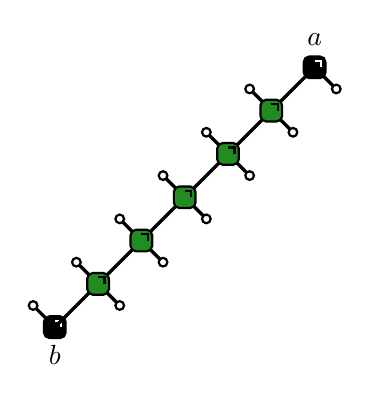
\begin{tikzpicture}[baseline=(current bounding box.center), scale=0.55]
\foreach \i in {1,...,5}
{\Wgategreen{3+\i}{\i}}
\foreach \i in {1,...,5}
{\MYcircle{2.5+\i}{0.5+\i}}
\foreach \i in {1,...,5}
{\MYcircle{3.5+\i}{-0.5+\i}}
\MYsquareB{3.0}{0}
\draw[very thick](3,0)--(3.5,0.5);
\draw[very thick](3,0)--(2.5,0.5);
\MYcircle{2.5}{0.5};
\MYsquareB{9}{6}
\draw[very thick](9,6)--(8.5,5.5);
\draw[very thick](9,6)--(9.5,5.5);
\MYcircle{9.5}{5.5};
\Text[x=3,y=-.65]{$b$}
\Text[x=9,y=6.65]{$a$}
\end{tikzpicture}
,\label{eq:support2lightcone}
\end{equation}
\begin{equation}
\braket{a_j(t) b_j}=
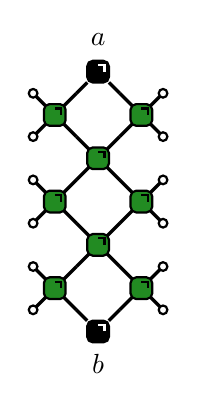
\begin{tikzpicture}[baseline=(current bounding box.center), scale=0.55]
\foreach \i in {1,2}
{
\Wgategreen{4}{2*\i}
\Wgategreen{3}{1+2*\i}
\Wgategreen{5}{1+2*\i}
\MYcircle{5.5}{1.5+2*\i}
\MYcircle{5.5}{0.5+2*\i}
\MYcircle{2.5}{1.5+2*\i}
\MYcircle{2.5}{0.5+2*\i}
}
\Wgategreen{3}{1}
\Wgategreen{5}{1}
\MYcircle{5.5}{1.5}
\MYcircle{5.5}{0.5}
\MYcircle{2.5}{1.5}
\MYcircle{2.5}{0.5}
\MYsquareB{4}{0}
\draw[very thick] (4.25,0.25) -- (4.5,0.5);
\draw[very thick] (3.75,0.25) -- (3.5,0.5);
\MYsquareB{4}{6}
\draw[very thick] (3.75,5.75) -- (3.5,5.5);
\draw[very thick] (4.25,5.75) -- (4.5,5.5);
\Text[x=4,y=-0.75]{$b$}
\Text[x=4,y=6.75]{$a$}
\end{tikzpicture}
. \label{eq:support2timeaxis}
\end{equation}
%\pk{Express using Q, algebraicallq the i,i case}
%
The correlation function in Eq. (\ref{eq:support2lightcone}) along the light cone is exactly the same as Eq. (\ref{eq:expression_CF_1site}).
By implementing the quantum channel defined as
\begin{equation}
\mathbb{Q}=
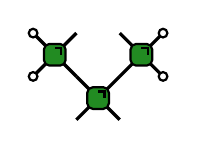
\begin{tikzpicture}[baseline=(current  bounding  box.center), scale=0.55]
\Wgategreen{0}{0}
\Wgategreen{-1}{1}
\Wgategreen{1}{1}
\MYcircle{-1.5}{1.5}
\MYcircle{-1.5}{0.5}
\MYcircle{1.5}{1.5}
\MYcircle{1.5}{0.5}
\end{tikzpicture},
\end{equation}
we can express Eq.~\eqref{eq:support2timeaxis} in a compact analytical form $C_{i,i}(t)=\begin{cases}
    \mathrm{Tr}(a\mathbb{Q}^tb), &t=\mathbb{Z},\\
    \mathrm{Tr}(aw\mathbb{Q}^tb), &t=\mathbb{Z}+\frac{1}{2}.\\
\end{cases}$

%where \begin{tikzpicture}[baseline=(current bounding box.center), scale=0.55]
%\MYsquareB{4}{0}
%\end{tikzpicture} represents the operator acting on two nearest neighbor sites.
%In Fig. (\ref{Correlation_func_sup2}), we present the correlation function for the operator supporting on multiple sites in different local dimensions. It is evident from the figure that the correlation function is nonzero exclusively along the three directions.

\begin{figure}
\includegraphics[width=0.9\columnwidth]{CFCtotalfigure}
\caption{(a) The correlation function for $D=6$ dimension, supporting on 2 sites. The gate is a non-ergodic member of $\overline{\mathfrak{L}}_2$ with parametrization given by Eq. (\ref{eq:simplest_2nd_Hierarchy_case}). 
(b) %The time $t$ and location $i$ are defined in Eq. (\ref{eq:definitionofcorrelationfunction}).
The correlation function for the qubit case supported on 3 sites. The gate is an ergodic element of $\overline{\mathfrak{L}}_2$, with parameters given in the Appendix \ref{app:parameters}. The asymmetry between the left and right sides results from even/odd effects.
In both figures, $a_{i}=b_{j}=h$, with $h$ a random normalized traceless Hermitian operator. 
$j$ is fixed at $20$. The location of a multi-site operator is defined as the location of its left end. 
%The color intensity in the graph represents the absolute value of the correlation function; the deeper the color, the larger the absolute value. 
}
\label{Correlation_func_sup2}
\end{figure}

Let us have a look at the correlation function's intriguing temporal decay. Generally speaking, the long-term behavior of the correlation function will be dominated by the largest eigenvalue $\lambda$ of the quantum channel, evolving as $\sim \lambda^t$~\footnote{The identity operator is trivially an eigenvector of the quantum channel with eigenvalue $1$, but it does not matter due to the tracelessness of initial operators.}. 
If $|\lambda|=1$, the correlation function will persist without decay. This behavior is referred to as non-ergodic. 
%
A simple example of $\overline{\mathfrak{L}}_2$ circuit in higher dimension, Eq. (\ref{eq:simplest_2nd_Hierarchy_case}) with $D=6,v_1=v_2=I_D$, falls into this class, as illustrated in Fig. \ref{Correlation_func_sup2}(a). Conversely, if $|\lambda|<1$, the correlation function will be ergodic and exhibit an exponential decay, a point we will come back later in Sec. \ref{Quantum_quench} in the context of quantum quenches. An ergodic example can also be constructed from Eq. (\ref{eq:simplest_2nd_Hierarchy_case}) by choosing $D=6,v_i=\sigma_x\otimes\kappa_i,i\in{1,2}$ for almost any $\kappa_i\in\mathbb{SU}(3)$.


The scenario with three sites operators  follows
 the preceding discussions without any additional difficulty. The correlators along the time axis can be expressed with the quantum channel 
 \begin{equation}
 \mathbb{R}=\begin{tikzpicture}[baseline=(current bounding box.center), scale=0.55]
\Wgategreen{0}{0}
\Wgategreen{2}{0}
\Wgategreen{-1}{1}
\Wgategreen{1}{1}
\MYcircle{2.5}{-0.5}
\MYcircle{2.5}{0.5}
\MYcircle{-1.5}{0.5}
\MYcircle{-1.5}{1.5}
\end{tikzpicture}.
\end{equation}
%
%According to the largest eigenvalue of the quantum channel, we can also distinguish the ergodic and non-ergodic case. 
Its largest non-trivial eigenvalue is typically smaller than $1$.
Fig. \ref{Correlation_func_sup2}(b) showcases this ergodic qubit circuit. We further examine the correlators at $i=j$ and $i=j+t$ in Fig. \ref{exponential_decay_CF}. %The evident exponential decay confirms the preceding argument. %Due to the even-odd effect and the interference among different eigenvectors, the correlation function along the time axis (i.e. when $i=j$) exhibits larger fluctuations\pk{which fluctuations do you have in mind?} than that along the time cone (i.e. when $i=j+t)$.


\begin{figure}
\includegraphics[width=0.9\columnwidth]{decay_of_correlationfunction}

\caption{This figure demonstrates the exponential decay of the correlation function along both the time axis (i.e., $i=j$) and the light cone (i.e., $i=t+j$). The two-qubit gate from $\overline{\mathfrak{L}}_2$, and the operators $a$ and $b$ are identical to the one used in Fig. \ref{Correlation_func_sup2}(b). The solid line represents a linear fit of the exponential decay.
}

\label{exponential_decay_CF}
\end{figure}

Moving beyond the scope of $2-$point correlation functions, $3-$point correlation functions provide more information of the non-equilibrium dynamics. They are defined as follows:
\begin{equation}
\begin{aligned}
C_{i,j,k}(t_{1},t_{2})=&\langle a_{i}(t_{1})b_{j}(t_{2})c_{k}\rangle\\
=D&\mathrm{Tr}\left((\mathbb{U}^\dagger)^{t_2}[(\mathbb{U}^\dagger)^{t_1-t_2}a_i\mathbb{U}^{t_1-t_2}b_j]\mathbb{U}^{t_2}c_k\frac{1}{D^{2L}}\right).
\end{aligned}
\end{equation}
If $i$ and $j$ are on the same side of $k$, the $3-$point correlation functions become trivial for $\mathfrak{L}_2$ circuits, i.e., either vanishes or reduces to $2-$point correlations.
\begin{comment}can be represented as follows: 

\begin{equation}
C_{i,j,k}(t_1,t_2)=
\begin{tikzpicture}[baseline=(current bounding box.center), scale=0.55]
\foreach \i in {0,...,4}
{
\Wgategreen{-\i}{\i}
\MYcircle{-\i-0.5}{\i-0.5}
}
\foreach \i in {0,...,4}
{
\Wgategreen{1-\i}{1+\i}
}
\foreach \i in{0,1,2}
{
\Wgategreen{2-\i}{2+\i}
\MYcircle{2.5-\i}{2.5+\i}
}
\MYcircle{1.5}{0.5}
\MYcircle{2.5}{1.5}
\MYcircle{-4.5}{4.5}
\MYcircle{-2.5}{5.5}
\MYcircle{-1.5}{4.5}
\MYcircleB{0.5}{-0.5}
\MYcircleB{-3.5}{5.5}
\MYcircleB{-0.5}{4.5}
\Text[x=0.5,y=-1]{$c$};
\Text[x=-3.5,y=6]{$a$};
\Text[x=-0.5,y=5]{$b$};
\end{tikzpicture}
.
\end{equation}
When related? to the $\mathfrak{L}_2$, this correlation function will disappear for traceless operators.
\end{comment}
%The $3-$point correlation functions only become nontrivial when $i$ and $j$ are located on different sides of $k$. 
Therefore, without loss of generality, we can assume $i<k<j$ such that
\begin{equation}
\begin{aligned}
&C_{i,j,k}(t_1,t_2)=\\
&\begin{tikzpicture}[baseline=(current bounding box.center), scale=0.55]
\Wgategreen{1}{5}
\foreach \i in {0,...,3}
{
\Wgategreen{0}{2*\i}
\Wgategreen{-1}{1+2*\i}
\Wgategreen{1+\i}{3+\i}
}
\foreach \i in {0,1,2}
{
\Wgategreen{-2-\i}{8+\i}
}
\MYcircle{0.5}{6.5}
\foreach \i in {0,...,6}
{
\MYcircle{-1.5}{.5+\i}
}
\foreach \i in {0,1}
{\MYcircle{3.5-\i}{6.5-\i}}
\foreach \i in {0,1,2}
{
\MYcircle{0.5}{\i-0.5}
\MYcircle{-2.5-\i}{7.5+\i}
}
\foreach \i in {0,...,3}
{
\MYcircle{1.5+\i}{2.5+\i}
\MYcircle{-0.5-\i}{7.5+\i}
}
\MYcircle{1.5}{5.5}
\MYcircleB{-0.5}{-0.5}
\MYcircleB{4.5}{6.5}
\MYcircleB{-4.5}{10.5}
\Text[x=-0.5,y=-1] {$c$}
\Text[x=4.5,y=7] {$b$}
\Text[x=-4.5,y=11] {$a$}
\draw[thick, dashed](5.5,6.5)--(7,6.5);
\draw[thick, dashed](5.5,-0.5)--(7,-0.5);
\Text[x=6.25,y=3]{$t_2$};
\draw[thick, dashed](-5.5,10.5)--(-7,10.5);
\draw[thick, dashed](-5.5,-0.5)--(-7,-0.5);
\Text[x=-6.25,y=5]{$t_1$};
\draw[->](6.25,3.5)--(6.25,6);
\draw[->](6.25,2.5)--(6.25,0);
\draw[->](-6.25,5.5)--(-6.25,10);
\draw[->](-6.25,4.5)--(-6.25,0);
\draw[thick, dashed](1,0)--(2,0);
\draw[thick, dashed](1,1)--(2,1);
\Text[x=3,y=0.5]{$t_2-(j-k)-\frac{1}{2}$};
\draw[thick, dashed](-5,0)--(-4,0);
\draw[thick, dashed](-5,6)--(-4,6);
\node at (-4.5,3) [rotate=-90] {$t_1-(k-i)-\frac{1}{2}$};
%\draw[->](-4.5,5.5)--(-4.5,5.5);
%\draw[->](-4.5,1)--(-4.5,0.5);
\draw[thick, dashed](-3,1)--(-2,1);
\draw[thick, dashed](-3,6)--(-2,6);
\node at (-2.5,3.5) {$l$};
\draw[->](-2.5,4)--(-2.5,5.5);
\draw[->](-2.5,3)--(-2.5,1.5);
\end{tikzpicture}
.\label{eq:3pointresult}
\end{aligned}
\end{equation}
Unlike the $\mathfrak{L}_1$, there are non-trivial correlation even when both $a$ and $b$ are strictly inside the light cone.

Nevertheless, despite the fact that the $\mathfrak{L}_2$ condition greatly simplifies the circuit complexity, it does not fully resolve all computational challenges. Viewing from Eq. (\ref{eq:3pointresult}) we obtain that the maximum number of qudits (legs) we need to store when contracting the graph diagonally is $l+\frac{1}{2}$ with $l$ labeled in Eq. (\ref{eq:3pointresult}), thus the computational complexity scales as $e^{\mathcal{O}(|(t_{1}-k+i)-(t_{2}-j+k)|)}$. %because the base length of the unsimplified triangle is $|(t_{1}-|i-k|)-(t_{2}-|j-k|)|$. 
%\pk{I still need to double check.}


\subsection{Quantum Quench in $\overline{\mathfrak{L}}_2$ circuits}
\label{Quantum_quench}

%\pk{We need to be careful with TD limit: say where we take it or need just t>L?}

In this subsection, we examine the correlation functions for $\overline{\mathfrak{L}}_2$ circuits following a quantum quench, i.e. originating from an initial density matrix $\rho_L(0)$. Here $\rho_L(0)$ can either be a pure state or a mixed state with a local purification.
Therefore we can write it with a local purifying Matrix Product State (MPS) as $\rho_{L}^A(0)=\mathrm{Tr}_{\gamma_{1},\cdots,\gamma_{L}}\ket{\Psi_{L}(A)}\bra{\Psi_{L}(A)}$ 
\cite{kos2023circuits,piroli2020exact}, where
\begin{equation}
\begin{aligned}\ket{\Psi_{L}(A)} & =\\
\sum_{\{i_{k}^{\mathrm{L}},i_{k}^{\mathrm{R}},\gamma_{k}\}} & \mathrm{Tr}\left(A^{(i_{1}^{\mathrm{L}}i_{1}^{\mathrm{R}}\gamma_{1})}\cdots A^{(i_{L}^{\mathrm{L}}i_{L}^{\mathrm{R}}\gamma_{L})}\right)\ket{i_{1}^{\mathrm{L}}i_{1}^{\mathrm{R}}\gamma_{1}\cdots i_{L}^{\mathrm{L}}i_{L}^{\mathrm{R}}\gamma_{L}}
\end{aligned}.
\end{equation}
Here $\gamma_i$ is the purification  index, which we sum over in $\rho_L(0)$.
Without additional specifications, the gates in this subsection are assumed to be from $\overline{\mathfrak{L}}_2$. %\pk{[We still need to vectorize this!, also later]}
 Graphically, the vectorized density matrix can be represented as 
\begin{equation}
\ket{\rho_L^A(0)}=\frac{1}{d^L} \;
\begin{tikzpicture}[baseline=(current bounding box.center), scale=0.55]
\draw[very thick] (-1.0 ,0.) -- (3.0,0.);
\rhoO{0}{0}\rhoO{2}{0}
\end{tikzpicture}
=
\begin{tikzpicture}[baseline=(current  bounding  box.center), scale=.7]
\def\dx{0.15}
\def\dy{0.15}
\draw[ thick] (-4.75+.2+\dx,0.+\dy) --(-0.0+0.2+\dx,0.+\dy);
%
\draw[ thick] (-3.75+\dx,0.75+\dy) -- (-3.75+\dx,-0.0+\dy);
\draw[ thick] (-3.25+\dx,0.75+\dy) -- (-3.25+\dx,0.0+\dy);
\draw[ thick, fill=myblue, rounded corners=2pt] (-4+\dx,0.25+\dy) rectangle (-2.5+\dx,-0.25+\dy);
%\draw[thick] (-3.75+\dx,0.15+\dy) -- (-3.75+0.15+\dx,0.15+\dy) -- (-3.75+0.15+\dx,0+\dy);
%----
\draw[ thick] (-1.75+\dx,0.75+\dy) -- (-1.75+\dx,-0.0+\dy);
\draw[ thick] (-1.25+\dx,0.75+\dy) -- (-1.25+\dx,0.0+\dy);
\draw[ thick, fill=myblue, rounded corners=2pt] (-2+\dx,0.25+\dy) rectangle (-0.5+\dx,-0.25+\dy);
\draw[ thick] (-2.75 ,0.25) -- (-2.75,0.25+.2) --(-2.75+\dx,0.25+\dy+.2) --(-2.75+\dx,0.25+\dy);
%Horizontal 
\draw[ thick] (-4.75 ,0.) -- (-.0+.2,0.);
\draw[ thick] (-3.75,0.75) -- (-3.75,-0.0);
\draw[ thick] (-3.25,-0.0) -- (-3.25,0.75);
\draw[ thick, fill=myorange0, rounded corners=2pt] (-4,0.25) rectangle (-2.5,-0.25);
\draw[ thick] (-1.75,0.75) -- (-1.75,-0.0);
\draw[ thick] (-1.25,-0.0) -- (-1.25,0.75);
\draw[ thick, fill=myorange0, rounded corners=2pt] (-2,0.25) rectangle (-0.5,-0.25);
%----
\draw[ thick] (-0.75 ,0.25) -- (-0.75,0.25+.2) --(-0.75+\dx,0.25+\dy+.2) --(-0.75+\dx,0.25+\dy);
%\Text[x=-3.65,y=0.75]{$i^L j^L$}
\end{tikzpicture} \; .
\end{equation}
%
A physically density matrix is normalized in the thermodynamic limit
\begin{equation}
\lim_{L\to\infty}\braket{I|\rho_L^A(0)}=\lim_{L\to\infty}\mathrm{Tr}E(0)^L=1,
\end{equation}
where $E(0)$ is the space transfer matrix
\begin{equation}
E(0)=\begin{tikzpicture}[baseline=(current bounding box.center), scale=0.55]
\rhoO{0}{0}
\MYcircle{-0.5}{0.5}
\MYcircle{0.5}{0.5}
\end{tikzpicture}.
\end{equation}
This implies that $E(0)$ has a unique non-degenerate left and right fixed point whose eigenvalue is one 
\begin{equation}
    \lim_{L\to\infty}E(0)^L=\ket{\square}\bra{\vartriangle}\label{eq:leftrightfixedpoint}
\end{equation}
with $\braket{\vartriangle|\square}=1$.
%
\subsubsection{$1-$point correlation functions}
%The properties of the initial state are inherited in the time evolution of $1-$point correlation function, which is defined as 
The most basic information about the dynamic from a quantum quench is contained in the $1-$point correlation function, which specifies the relaxation and thermalization of local observables. It is defined as
\begin{equation}
\lim_{L\to\infty}\braket{O_1|\rho_L(t)}=\lim_{k\to\infty}\mathrm{Tr}(E^{k}(t)E_{O_{1}}(t)E^{k}(t)).
\end{equation}
Here, $E(t)=E_{\1}(t)$ and $E_{O_{1}}(t)$ are appropriate space transfer matrices
%
\begin{equation}
\begin{aligned}
\braket{O_1|\rho_L(t)} & =
\begin{tikzpicture}[baseline=(current bounding box.center), scale=0.55]
\draw [very thick] (-0.5,0) -- (6.5,0);
\foreach \i in {0,2,4,6}
{\rhoO{\i}{0}}
\foreach \i in {1,3,5}
{
\foreach \j in {1,3}
{
\Wgategreen{\i}{\j}
}
}
\foreach \i in {0,2,4,6}
{
\foreach \j in {2,4}
{
\Wgategreen{\i}{\j}
}
}
\foreach \i in {0,1,2,3,5,6,7}
{
\MYcircle{\i-0.5}{4.5}
}
\MYcircleB{3.5}{4.5}
\Text[x=3.5,y=5] {$O_1$};
\draw[gray, dashed](2.7,4.65)--(2.7,-0.15)--(4.7,-0.15)--(4.7,4.65)--cycle;
\Text[x=3.5,y=-.65] {$E_{O_1}$(t)};
\end{tikzpicture}
. 
\end{aligned}
.
\end{equation}
In this subsection we always assume periodic boundary conditions with large enough $L$ such that the transfer matrix can be replaced by its fixed point. 

If the initial state satisfies the following \emph{$1-$point solvable
condition for $\overline{\mathfrak{L}}_2$}
\begin{equation}
\begin{tikzpicture}[baseline=(current bounding box.center), scale=0.55]
\rhoO{0}{0}
\Wgategreen{-1}{1}
\MYcircle{-0.5}{1.5}
\MYcircle{0.5}{0.5}
\MYsquare{0.5}{0}
\end{tikzpicture}
=
\begin{tikzpicture}[baseline=(current bounding box.center), scale=0.55]
\draw[very thick] (-0.5,0) -- (0.5,0);
\Wgategreen{-1}{1}
\MYcircle{-0.5}{1.5}
\MYcircle{-0.5}{0.5}
\MYsquare{0.5}{0}
\end{tikzpicture}
, \label{eq:transfer_condi}
\end{equation}
we can find an eigenstate of the transfer matrix with eigenvalue $1$ 
\begin{equation}
\begin{tikzpicture}[baseline=(current bounding box.center), scale=0.55]
\rhoO{-1}{0}
\foreach \j in {1,3}
{
\Wgategreen{-2}{\j}
}
\foreach \j in {2,4}
{
\Wgategreen{-1}{\j}
}
\MYcircle{-1.5}{4.5}
\MYcircle{-0.5}{4.5}
\draw[very thick] (-0.5,0)--(0.5,0);
\MYsquare{0.5}{0}
\foreach \j in {1,3}
{
\Wgategreen{0}{\j}
}
\foreach \j in {1,2,3,4}
{
\MYcircle{0.5}{\j-0.5}
}
\draw[gray, dashed] (-2.5,-0.15)--(-0.35,-0.15)--(-0.35,4.65)--(-2.5,4.65)--cycle;
\Text[x=-1.5,y=-.65]{$E(t)$};
\end{tikzpicture}
\;
=
\;
\begin{tikzpicture}[baseline=(current bounding box.center), scale=0.55]
\draw[very thick] (-0.5,0)--(0.5,0);
\MYsquare{0.5}{0}
\foreach \j in {1,3}
{
\Wgategreen{0}{\j}
}
\foreach \j in {1,2,3,4}
{
\MYcircle{0.5}{\j-0.5}
}
\end{tikzpicture}
.
\end{equation}
Since $\lim_{L\to\infty}\mathrm{Tr}(\rho_L(t))=1$ due
to the normalization, the largest eigenvalue of the trasnfer matrix
must be $1$ and non-degenerate. Therefore, the $1-$point correlation
function can be analytically calculated with this eigenvector.


It is worth to note that if the initial state satisfies the condition 
$\begin{tikzpicture}[baseline=(current bounding box.center), scale=0.55]
\rhoO{0}{0}
\MYcircle{0.5}{0.5}
\MYsquare{0.5}{0}
\end{tikzpicture}
\;
=
\begin{tikzpicture}[baseline=(current bounding box.center), scale=0.55]
\draw[very thick] (-0.5,0) -- (0.5,0);
\draw[very thick] (-0.5,0.5) -- (0.5,0.5);
\MYcircle{0.5}{0.5}
\MYsquare{0.5}{0}
\end{tikzpicture}
\,
,$ Eq. (\ref{eq:transfer_condi}) is automatically satisfied. This implies
that we have identified a larger solvable class than both the pure solvable initial states for dual-unitary evolution~\cite{piroli2020exact} and in general mixed initial states for open 3-way unital evolution~\cite{kos2023circuits}.


The correlation function for $2-$site observables after a quench is very similar to Eq. (\ref{eq:support2timeaxis}). The only difference is the substitution of $\begin{tikzpicture}[baseline=(current  bounding  box.center), scale=0.45]
\MYsquareB{0}{0}
\draw[very thick](0.25,0.25)--(0.5,0.5);
\draw[very thick](-0.25,0.25)--(-0.5,0.5);
\end{tikzpicture}$ at the base for 
$\begin{tikzpicture}[baseline=(current  bounding  box.center), scale=0.55]
\rhoO{0}{0}
\MYsquare{0.5}{0}
\MYtriangle{-0.5}{0}
\end{tikzpicture}$.
%
\begin{equation}
\braket{O_1|\rho_L(t)} =\begin{tikzpicture}[baseline=(current bounding box.center), scale=0.55]
\foreach \i in {1,2}
{
\Wgategreen{4}{2*\i}
\Wgategreen{3}{1+2*\i}
\Wgategreen{5}{1+2*\i}
\MYcircle{5.5}{1.5+2*\i}
\MYcircle{5.5}{0.5+2*\i}
\MYcircle{2.5}{1.5+2*\i}
\MYcircle{2.5}{0.5+2*\i}
}
\Wgategreen{3}{1}
\Wgategreen{5}{1}
\MYcircle{5.5}{1.5}
\MYcircle{5.5}{0.5}
\MYcircle{2.5}{1.5}
\MYcircle{2.5}{0.5}
\rhoO{4}{0}
\MYsquare{4.5}{0}
\MYtriangle{3.5}{0}
\draw[very thick] (4.25,0.25) -- (4.5,0.5);
\draw[very thick] (3.75,0.25) -- (3.5,0.5);
\MYsquareB{4}{6}
\draw[very thick] (3.75,5.75) -- (3.5,5.5);
\draw[very thick] (4.25,5.75) -- (4.5,5.5);
\Text[x=4,y=6.75]{$O_1$}
\end{tikzpicture},
\end{equation}
where $\bra{\vartriangle}$ and $\ket{\square}$ are the left and right fixed points from Eq. (\ref{eq:leftrightfixedpoint}). Following the same argument as in Sec. \ref{subsec:Biggersupports}, the long time behavior is dictated by the largest eigenvalue of the quantum channel, $\mathbb{Q}$. The eigenspectrum of $\mathbb{Q}$ can be completely deduced for qubits. Using the general parametrization of gates from $\overline{\mathfrak{L}}_2$ in accordance with Eqs. (\ref{eq:parameter2qubit}) and (\ref{eq:condition2ndqubit}), whereby $v_{3}=v_{4}=I$, $\theta_{i}=\arcsin{\frac{1}{\sqrt{2}\sin{r_{i}}}},i\in\{1,2\}$, only two non-zero eigenvalues, $\{1,\lambda\}$, exist. Eigenvalue $1$ corresponds to the trivial eigenvector, i.e. identity and $\lambda$ is given by
\begin{equation}
\begin{aligned}
&\lambda=\cos^2{(\phi_2-\phi_1)}\\
&-2(\sqrt{-\cos{2r_2}}\cos{r_1}+\sqrt{-\cos{2r_1}}\cos{r_2})^2.
\label{eq:quantumquenchchannel2qubit}
\end{aligned}
\end{equation}
Here $r_1,r_2$ are real numbers from the interval $[\frac{\pi}{4},\frac{3\pi}{4}]$.

The dynamics is non-ergodic with $\lambda=1$ if $\phi_1=\phi_2+0,\pi$ and either $r_1=\pi-r_2$ or $\cos{2r_1}=\cos{2r_2}=0$. On the other hand, the circuit is non-ergodic also with $\lambda=-1$ if $\cos(\phi_1-\phi_2)=0$ and the last term in Eq. (\ref{eq:quantumquenchchannel2qubit}) equals $1$, for example, by $r_1=\frac{\pi}{2},r_2=\frac{\pi}{4}$. This gives all possible non-ergodic circuits for two-qubit gates from $\overline{\mathfrak{L}}_2$, apart from a tensor product of single-site gates. All other examples are ergodic and show exponential decay.

\begin{figure}
\includegraphics[width=0.9\columnwidth]{thermal_quantum_quench}

\caption{The correlation function of a random two-site observable following a quantum quench starting from the Bell state $\ket{\Psi_L}$ defined in Eq. (\ref{eq:manybodyinitialstate}). The dynamics is governed by a $\overline{\mathfrak{L}}_2$ circuit (symbols). We show its linear fit by solid lines.
%The solid line represents the linear fitting curve. 
The blue and green data points show an exponential decay of the expectation value of observable, indicative of thermalization dynamics. In contrast, the red points remains constant at long times implying non-thermalization and non-ergodicity. The parameters for these three circuits can be found in Appendix~\ref{app:parameters}.
}
\label{quench_correlation}
\end{figure}

The most straightforward solution of initial states from Eq. (\ref{eq:transfer_condi}) is the pure state with a bond dimension $1$. One example is the qubit Bell state
\begin{equation}
\ket{\Psi_L}=\otimes_{k=1}^L\frac{\ket{01}_{2k-1,2k}+\ket{10}_{2k-1,2k}}{\sqrt{2}},
\label{eq:manybodyinitialstate}
\end{equation}
which we use in Fig.~\ref{quench_correlation}, where we show both thermalizing and non-thermalizing behaviors.
In contrast to the situation here, for $\mathfrak{L}_1$ (dual-unitarity) the expectation values of local observables trivially vanish at all times, even for clearly non-ergodic circuits such as circuits made out of SWAPs.
%
%Three $\overline{\mathfrak{L}}_2$ Hierarchical circuits with distinct behavior are shown in Fig. \ref{quench_correlation}. 






\subsubsection{$2-$point correlation functions}
Finally, we are moving to the $2-$point correlation functions after a quench, which are non trivial even for the $\mathfrak{L}_1$~\cite{piroli2020exact}.
Diagrammatically they  are represented as
\begin{align}\label{eq:quench2}
&C_{ij}(t) = 
\begin{tikzpicture}[baseline=(current  bounding  box.center), scale=0.55]
\foreach \i in {0,...,1}
{
\Wgategreen{-2}{0+2*\i}
\Wgategreen{0}{0+2*\i}
%\Wgategreen{2}{0+2*\i}
\Wgategreen{4}{0+2*\i}
\Wgategreen{6}{0+2*\i}
%\Wgategreen{8}{0+2*\i}
\Wgategreen{-1}{1+2*\i}
\Wgategreen{1}{1+2*\i}
%\Wgategreen{3}{1+2*\i}
\Wgategreen{5}{1+2*\i}
\Wgategreen{7}{1+2*\i}
%\Wgategreen{9}{1+2*\i}
}
\Text[x=2.5,y=1.5]{$\cdots$};
\Text[x=2.5,y=-1]{$\cdots$};
\draw[very thick] (-2.25,-1) -- (2,-1);
\draw[very thick] (3,-1) -- (7.5,-1);
\foreach \i in {2.5,4.5,8.5,10.5}
{\rhoO{-3.5+\i}{-1}}
%  
\foreach \i in {-1,0,1,2,5,6,7,8}
{ 
\draw[thick, fill=white] (\i-0.5,4-0.5) circle (0.1cm);
}
\MYcircleB{7.5}{3.5}
\MYcircleB{-1.5}{3.5}
\Text[x=-1.5,y=4.0]{$a$}
\Text[x=7.5,y=4.0]{$b$}
\end{tikzpicture}
.
\end{align} 

By leveraging time unitarity, we can deduce the emergence of two backward propagating light cones originating from the operators, interconnected by the initial state's transfer matrix $E(0)$
%
\begin{widetext}
\begin{align}
C_{ij}(t)=
\begin{tikzpicture}[baseline=(current  bounding  box.center), scale=0.55]
\Wgategreen{-8}{0}
\Wgategreen{-6}{0}
\Wgategreen{-4}{0}
\Wgategreen{-2}{0}
\Wgategreen{4}{0}
\Wgategreen{6}{0}
\Wgategreen{8}{0}
\Wgategreen{10}{0}
%
\Wgategreen{-5}{3}
\Wgategreen{7}{3}
\Wgategreen{-6}{2}
\Wgategreen{-4}{2}
\Wgategreen{6}{2}
\Wgategreen{8}{2}
\Wgategreen{-7}{1}
\Wgategreen{-5}{1}
\Wgategreen{-3}{1}
\Wgategreen{5}{1}
\Wgategreen{7}{1}
\Wgategreen{9}{1}
%
\draw[very thick] (-10.5,-1) -- (13.5,-1);
\draw[very thick,dotted] (-12.5,-1) -- (-10.5,-1);
\draw[very thick,dotted] (13.5,-1) -- (14.5,-1);
\foreach \i in {-7.5,-5.5,-3.5,-1.5,0.5,2.5,4.5,6.5,8.5,10.5,12.5,14.5,16.5}
{ \rhoO{-3.5+\i}{-1} }
%
\foreach \i in {0,...,3}
{
\MYcircle{\i-4.5}{3.5-\i}
\MYcircle{\i+4-.5}{0.5+\i}
\MYcircle{\i-.5+8}{3.5-\i}
\MYcircle{\i-4-4.5}{0.5+\i}
}
\MYcircle{-9.5}{-.5}  
\MYcircle{-10.5}{-.5} 
\MYcircle{-11.5}{-.5}
\MYcircle{11.5}{-.5}  
\MYcircle{12.5}{-.5}  
\MYcircle{13.5}{-.5} 
\MYcircle{2.5}{-0.5}
\MYcircle{1.5}{-0.5}
\MYcircle{0.5}{-0.5}
\MYcircle{-0.5}{-0.5}
\MYcircleB{7.5}{3.5} 
\MYcircleB{-5.5}{3.5}
\Text[x=-5.5,y=4.0]{$a$}
\Text[x=7.5,y=4.0]{$b$}
\end{tikzpicture}.
\label{eq:quench4}
\end{align}
\end{widetext} 
The number of repetitions of the transfer matrices $E(0)$ in the central region
depends on the separation, given by $j-i-(t_{1}+t_{2})+\frac{1}{2}$. The suitable 
\emph{$\mathfrak{L}_2$ 2-point correlator solvability condition} for this correlation function is 
\begin{equation}
\begin{tikzpicture}[baseline=(current  bounding  box.center), scale=0.55]
\rhoO{0}{0}
\MYsquare{0.5}{0}
\MYcircle{0.5}{0.5}
\end{tikzpicture}
=
\begin{tikzpicture}[baseline=(current  bounding  box.center), scale=0.6]
\draw[very thick] (-0.5,0) -- (0.5,0);
\draw[very thick] (-0.5,0.5) -- (0.5,0.5);
\MYsquare{0.5}{0}
\MYcircle{0.5}{0.5}
\end{tikzpicture}\;
;
\qquad
\begin{tikzpicture}[baseline=(current  bounding  box.center), scale=0.6]
\rhoO{0}{0}
\MYsquare{0.5}{0}
\Wgategreen{1}{1}
\MYcircle{1.5}{1.5}
\MYcircle{1.5}{0.5}
\end{tikzpicture}
=
\begin{tikzpicture}[baseline=(current  bounding  box.center), scale=0.55]
\draw[very thick] (-0.5,0) -- (0.5,0);
\draw[very thick] (-0.5,0.5) -- (0.5,0.5);
\draw[very thick] (-0.5,1.5) -- (0.5,1.5);
\MYsquare{0.5}{0}
\MYcircle{0.5}{0.5}
\MYcircle{0.5}{1.5}
\end{tikzpicture}\;
,\label{eq:solvable2points}
\end{equation}
and similar expression from left
\begin{equation}
\begin{tikzpicture}[baseline=(current  bounding  box.center), scale=0.55]
\rhoO{0}{0}
\MYtriangle{-0.5}{0}
\MYcircle{-0.5}{0.5}
\end{tikzpicture}
=
\begin{tikzpicture}[baseline=(current  bounding  box.center), scale=0.6]
\draw[very thick] (-0.5,0) -- (0.5,0);
\draw[very thick] (-0.5,0.5) -- (0.5,0.5);
\MYtriangle{-0.5}{0}
\MYcircle{-0.5}{0.5}
\end{tikzpicture}\;
;
\qquad
\begin{tikzpicture}[baseline=(current  bounding  box.center), scale=0.6]
\rhoO{0}{0}
\MYtriangle{-0.5}{0}
\Wgategreen{-1}{1}
\MYcircle{-1.5}{1.5}
\MYcircle{-1.5}{0.5}
\end{tikzpicture}
=
\begin{tikzpicture}[baseline=(current  bounding  box.center), scale=0.55]
\draw[very thick] (-0.5,0) -- (0.5,0);
\draw[very thick] (-0.5,0.5) -- (0.5,0.5);
\draw[very thick] (-0.5,1.5) -- (0.5,1.5);
\MYtriangle{-0.5}{0}
\MYcircle{-0.5}{0.5}
\MYcircle{-0.5}{1.5}
\end{tikzpicture}\;
.\label{eq:solvable2pointsleft}
\end{equation}
Here $\ket{\vartriangle}$ and $\ket{\square}$ are the left and right unique fixed point from Eq. (\ref{eq:leftrightfixedpoint}). %with eigenvalue $1$ of $E(0)$ normalizated as $\braket{\vartriangle|\square}=1$. 
Note that this condition is stronger than the solvability condition for the 1-point correlators. 
Following the same argument in~\cite{kos2023circuits}, it can be shown that any MPDO in the local purification form fulfilling solvability condition can be cast in right canonical form, which we use.
%Without loss of generality, we can choose the solvable state to be a right canonical tensor
Thus \begin{tikzpicture}[baseline=(current  bounding  box.center), scale=0.55]
\draw[very thick] (-0.,0) -- (0.5,0);
\MYsquare{0.5}{0}
\end{tikzpicture} is replaced by \begin{tikzpicture}[baseline=(current  bounding  box.center), scale=0.55]
\draw[very thick] (-0.,0) -- (0.5,0);
\MYcircle{0.5}{0}
\end{tikzpicture} (vectorized identity).

Supposing that the length $L$ is large enough, we can replace the outer parts of Eq. (\ref{eq:quench4}) by Eq. (\ref{eq:leftrightfixedpoint}).
After this simplification, we obtain
\begin{widetext}
\begin{align}
C_{ij}(t)=
\begin{tikzpicture}[baseline=(current  bounding  box.center), scale=0.55]
\Wgategreen{-8}{0}
\Wgategreen{-6}{0}
\Wgategreen{-4}{0}
\Wgategreen{-2}{0}
\Wgategreen{4}{0}
\Wgategreen{6}{0}
\Wgategreen{8}{0}
\Wgategreen{10}{0}
%
\Wgategreen{-5}{3}
\Wgategreen{7}{3}
\Wgategreen{-6}{2}
\Wgategreen{-4}{2}
\Wgategreen{6}{2}
\Wgategreen{8}{2}
\Wgategreen{-7}{1}
\Wgategreen{-5}{1}
\Wgategreen{-3}{1}
\Wgategreen{5}{1}
\Wgategreen{7}{1}
\Wgategreen{9}{1}
%
\draw[very thick] (-8.5,-1) -- (11.5,-1);
\foreach \i in {-5.5,-3.5,-1.5,0.5,2.5,4.5,6.5,8.5,10.5,12.5,14.5}
{ \rhoO{-3.5+\i}{-1} }
%
\foreach \i in {0,...,3}
{
\MYcircle{\i-4.5}{3.5-\i}
\MYcircle{\i+4-.5}{0.5+\i}
\MYcircle{\i-.5+8}{3.5-\i}
\MYcircle{\i-4-4.5}{0.5+\i}
}
\MYcircle{-9.5}{-.5}  
\MYcircle{11.5}{-.5}  
\MYcircle{2.5}{-0.5}
\MYcircle{1.5}{-0.5}
\MYcircle{0.5}{-0.5}
\MYcircle{-0.5}{-0.5}
\MYcircleB{7.5}{3.5} 
\MYcircleB{-5.5}{3.5}
\Text[x=-5.5,y=4.0]{$a$}
\Text[x=7.5,y=4.0]{$b$}
\MYtriangle{-9.5}{-1}
\MYcircle{11.5}{-1}
\end{tikzpicture}.
\label{eq:quench5}
\end{align}
\end{widetext} 
The leftmost and rightmost corners can be further reduced by the first equations from (\ref{eq:solvable2points}) and (\ref{eq:solvable2pointsleft}). Then with the help of the second equations from (\ref{eq:solvable2points}), (\ref{eq:solvable2pointsleft}) and the contraction properties of the $\overline{\mathfrak{L}}_2$, we arrive at 
\begin{align}
C_{ij}(t)=
\begin{tikzpicture}[baseline=(current  bounding  box.center), scale=0.55]
\Wgategreen{-4}{0}
\Wgategreen{-2}{0}
\Wgategreen{4}{0}
\Wgategreen{6}{0}
%
\Wgategreen{-5}{3}
\Wgategreen{7}{3}
\Wgategreen{-4}{2}
\Wgategreen{6}{2}
\Wgategreen{-5}{1}
\Wgategreen{-3}{1}
\Wgategreen{5}{1}
\Wgategreen{7}{1}
%
\draw[very thick] (-5,-1) -- (7,-1);
\foreach \i in {-1.5,0.5,2.5,4.5,6.5,8.5,10.5}
{ \rhoO{-3.5+\i}{-1} }
%
\foreach \i in {0,...,3}
{
\MYcircle{\i-4.5}{3.5-\i}
\MYcircle{\i+4-.5}{0.5+\i}
}
\foreach \i in {0,1,2,3}
{
\MYcircle{-5.5}{\i-0.5}
\MYcircle{7.5}{\i-0.5}
}
\MYtriangle{-5.5}{-1}
\MYcircle{7.5}{-1}
\MYcircle{2.5}{-0.5}
\MYcircle{1.5}{-0.5}
\MYcircle{0.5}{-0.5}
\MYcircle{-0.5}{-0.5}
\MYcircleB{7.5}{3.5} 
\MYcircleB{-5.5}{3.5}
\Text[x=-5.5,y=4.0]{$a$}
\Text[x=7.5,y=4.0]{$b$}
\end{tikzpicture}.
\label{eq:quench4_2}
\end{align}
Applying the first equation from (\ref{eq:solvable2points}), we finally
obtain a considerably simplified expression
\begin{equation}
C_{ij}(t)=
\begin{tikzpicture}[baseline=(current  bounding  box.center), scale=0.55]
\draw[very thick](-4,0)--(0,0);
\rhoO{0}{0}
\rhoO{-2}{0}
\rhoO{-4}{0}
\foreach \i in {1,2,3,4}
{
\Wgategreen{\i}{\i}
\Wgategreen{-\i-4}{\i}
\MYcircle{\i-0.5}{\i+0.5}
\MYcircle{\i+0.5}{\i-0.5}
\MYcircle{0.5-\i-4}{\i+0.5}
\MYcircle{-0.5-\i-4}{\i-0.5}
}
\foreach \i in {0,1,2,3}
{
\MYcircle{-\i-0.5}{0.5}
}
\MYcircle{0.5}{0}
\MYtriangle{-4.5}{0}
\MYcircleB{4.5}{4.5}
\MYcircleB{-8.5}{4.5}
\Text[x=4.5,y=5]{$b$}
\Text[x=-8.5,y=5]{$a$}
\end{tikzpicture}.
\end{equation}
%
Interestingly, if the separation $j-i$ is shorter than $t_{1}+t_{2}$,
the correlation function will vanish for traceless operators, which is the same as for $\mathfrak{L}_1$~\cite{piroli2020exact}.


Solvability condition from Eq. (\ref{eq:solvable2points}) can also be formulated in an algebraic form.
If we define an operator $K_{\gamma}$ as
\begin{equation}
K^{\dagger}_{\gamma}:=\sum_{i^{\mathrm{L}}j^{\mathrm{R}}}A^{(i^{\mathrm{L}}j^{\mathrm{R}}\gamma)}\otimes|i^{\mathrm{L}}\rangle\langle j^{\mathrm{R}}|,
\end{equation} 
% and replace
% \begin{tikzpicture}[baseline=(current  bounding  box.center), scale=0.55]
% \draw[very thick] (-0.5,0) -- (0.5,0);
% \MYsquare{0.5}{0}
% \end{tikzpicture} by \begin{tikzpicture}[baseline=(current  bounding  box.center), scale=0.55]
% \draw[very thick] (-0.5,0) -- (0.5,0);
% \MYcircle{0.5}{0}
% \end{tikzpicture}  for simplicity,
the solvability condition for an initial state in the right canonical form can be written as
\begin{equation}
\begin{aligned}\sum_{\gamma}K_{\gamma}^{\dagger}K_{\gamma} & =\frac{I_{d\chi}}{d};\\
\sum_{\gamma}I_{d}\otimes K_{\gamma}^{\dagger}(\tilde{U^{\dagger}}\tilde{U}\otimes I_{\chi})K_{\gamma}\otimes I_{d} & =\frac{I_{d^{2}\chi}}{d}.
\end{aligned}
\end{equation}
The same discussion holds from the left side, except that we need to keep $\ket{\vartriangle}$ instead of $\ket{\mcirc}$. 

For example, where the initial state is pure, that is, without summation
over $\gamma$, the first equation implies that $K$ is proportional
to a unitary operator. This leads to the conclusion that $U$ is a $\mathfrak{L}_1$, as per the second equation. Consequently, a solvable initial
state for $\overline{\mathfrak{L}}_2$ can only be a mixed state. As an example, if we choose $U=\mathrm{CNOT}$ and the bond dimension for
MPS to be $1$, a nontrivial solution is $K_{0}=\frac{I}{2\sqrt{2}},K_{1}=\frac{\sigma_{Y}}{2\sqrt{2}}$.
% Here $\sigma_{Y}=\begin{pmatrix}0 & -i\\
% i & 0
% \end{pmatrix}$.

%We would like to mention that a comparable method used for handling $2-$point correlation functions can also be applied to $1-$point correlation function. This results in the same solvable condition as expressed in (\ref{eq:transfer_condi}).

%------------------------

%-------------------------------------------------------------------------------------------------
\section{Conclusions and perspectives}
\label{sec:conclusions}
%In this paper, we have effectively broadened the scope of the dual-unitary circuits, extending them to a larger solvable classes referred to as Hierarchicals\pk{update}. These classes of circuits with comparatively relaxed conditions exhibit richer physical properties. Most intriguingly, their correlation functions are non-zero in the third direction. Furthermore, these circuits enable the exploration of the thermalization dynamics of quenched operators, a feat unachievable with the standard dual-unitary circuit. 

In this paper, we have generalized dual-unitary circuits to larger solvable classes referred to as levels of the Hierarchy. These families of circuits with comparatively relaxed conditions exhibit richer physical properties than the dual-unitary ones. Most intriguingly, their correlation functions are non-zero at the initial site and later times. Furthermore, these circuits show  nontrivial thermalization of local operators, in contrast with the standard dual-unitary circuit. 

In our work we provide the complete parametrization of $\mathfrak{L}_1,\mathfrak{L}_2,\mathfrak{L}_3$ for qubit circuits. For local dimensions bigger than two, we propose a systematic approach using the Clifford group to construct novel examples, which include both ergodic and nonergodic instances.


It is worth mentioning that even though we focus on the translational invariant dynamics, the results and methods presented do not depend crucially on this property and can be extended to time and space inhomogeneous settings. 
This study, therefore, provides a strong foundation for further explorations in the realm of solvable models and their real-world applications. 
They can be directly implemented on current NISQ devices, and used as benchmarks in the realms where ordinary classical simulations are no longer possible.
%The concepts and methodologies proposed in this study can be directly extended to scenarios where spatial and/or temporary inhomogeneous or randomness are incorporated. 

We mentioned that one interesting example is the CNOT gate and its extensions. They are a particular cases of Floquet East model, which shows interesting physics, e.g. hydrophobicity and localization, both in classical~\cite{klobas2023exact} and quantum realm~\cite{bertini2023localised}.
Interestingly, for a subset of the solvable $\mathfrak{L}_2$ connected to CNOT,  exact solutions can also be obtained using the so called zipper equations~\cite{klobas2021exact} by devising an exact eigenvectors of the transfer matrix~\cite{unpublished}. 

Of course, the ideas presented here can be extended to conditions on bunch of gates in different configurations from the ones presented here.
%One interesting observation extends beyond the confines of the brickwall circuits, indicating that the quantum circuits with alternative geometric configurations, such as the 
One direct way is generalizing the dual-unitarity
round-a-face~\cite{prosen2021manybody}. It is feasible to define the $\mathfrak{L}_2$ condition in this context as
\begin{equation}
\begin{tikzpicture}[baseline=(current  bounding  box.center), scale=0.55]
\draw[very thick, fill=mygreen,rounded corners=2pt](0,0.5)--(0.5,0)--(0,-0.5)--(-0.5,0)--cycle;
\draw[very thick,fill=mygreen,rounded corners=2pt](-0.5,0)--(0,-0.5)--(-0.5,-1)--(-1,-0.5)--cycle;
\MYcircle{0}{0.5}
\MYcircle{0.5}{0}
\MYcircle{0}{-0.5}
\MYcircle{-0.5}{-1}
\end{tikzpicture}
=
\begin{tikzpicture}[baseline=(current  bounding  box.center), scale=0.55]
\draw[very thick,fill=mygreen,rounded corners=2pt](-0.5,0)--(0,-0.5)--(-0.5,-1)--(-1,-0.5)--cycle;
\draw[very thick](-1,0.5)--(-0.5,0.5);
\MYcircle{-0.5}{0.5}
\MYcircle{-0.5}{0}
\MYcircle{0}{-0.5}
\MYcircle{-0.5}{-1}
\end{tikzpicture}.
\end{equation}
We anticipate these circuits to exhibit similar features as the $\mathfrak{L}_2$ circuits discussed here. For examples, their correlation functions might exclusively exist along three directions. However, parametrization of these types of circuits and their subsequent physical applications represent an intriguing path for future research.

One can also be  more bold, and demand for instance the following conditions:
	\begin{eqnarray}
		\begin{tikzpicture}[baseline=(current  bounding  box.center), scale=0.7]
			\Wgategreen{0}{1}
			\Wgategreen{1}{0}
			\Wgategreen{0}{-1}
			\Wgategreen{-1}{0}
			\Wgategreen{1}{-2}
			\MYcircle{1.5}{0.5}
			\MYcircle{1.5}{-0.5}
			\MYcircle{1.5}{-1.5}
			\MYcircle{1.5}{-2.5}
			\MYcircle{0.5}{1.5}
		\end{tikzpicture}&=&
		\begin{tikzpicture}[baseline=(current  bounding  box.center), scale=0.7]
	\Wgategreen{0}{1}
\Wgategreen{0}{-1}
\Wgategreen{-1}{0}
\Wgategreen{1}{-2}
\MYcircle{.5}{0.5}
\MYcircle{.5}{-0.5}
\MYcircle{1.5}{-1.5}
\MYcircle{1.5}{-2.5}
\MYcircle{0.5}{1.5}
		\end{tikzpicture},\nonumber\\
		\begin{tikzpicture}[baseline=(current  bounding  box.center), scale=0.7]
		\Wgategreen{0}{-1}
		\Wgategreen{-1}{0}
		\Wgategreen{0}{1}
		\Wgategreen{1}{0}
		\Wgategreen{-1}{2}
		\MYcircle{-1.5}{-0.5}
		\MYcircle{-1.5}{0.5}
		\MYcircle{-1.5}{1.5}
		\MYcircle{-1.5}{2.5}
		\MYcircle{-0.5}{-1.5}
		\end{tikzpicture}&=&
		\begin{tikzpicture}[baseline=(current  bounding  box.center), scale=0.7]
		\Wgategreen{0}{-1}
		\Wgategreen{0}{1}
		\Wgategreen{1}{0}
		\Wgategreen{-1}{2}
		\MYcircle{-0.5}{-0.5}
		\MYcircle{-0.5}{0.5}
		\MYcircle{-1.5}{1.5}
		\MYcircle{-1.5}{2.5}
		\MYcircle{-0.5}{-1.5}
%
  \Text[x=-0,y=-2]{$ $}
		\end{tikzpicture}.
	\end{eqnarray}

 
It can be shown, using a simplification procedure similar to that in Sec.~\ref{subsec:STCF}, that this condition leads to the exact solvability of two point spatial-temporal correlation functions in the region $-t/3<x<0$. This is interesting since it gives us a 2D space-time region where the spatial-temporal correlation functions are solvable and non-vanishing, while all dual-unitary circuits and their $\mathfrak{L}_2$ generalization have vanishing spatial-temporal correlations except on a few lines. Unfortunately, to date, we have not yet been able to find a nontrivial unitary gate satisfying this condition, due to the computational difficulty of solving this equation. We leave this possibility as an open direction for the future.

%\pk{Do we wish to discuss the Zhiyuan's suggested generalization here, even though we have no examples?}
%-------------------------------------------------------------------------------------------------
\section*{Acknowledgements}
We thank Ignacio Cirac, Katja Klobas, Bruno Bertini and Alessandro Foligno  for fruitful discussions.
PK is supported by the Alexander von Humboldt Foundation.
\vspace{.5cm}
%-------------------------------------------------------------------------------------------------


\appendix
\section{The parametrization of the Hierarchical gates in higher dimensions}\label{sec:appendixA}

In this appendix, we provide further details about deriving Eq. (\ref{eq:Clifford_parametrization_2nd_result}). In particular, inserting Eqs. (\ref{eq:2quditUgeneralform}) and (\ref{eq:CliffordParametrization}) into the first equation of (\ref{eq2:bottomtotop})
with $v_{3}=v_{4}=I_{D}$, we obtain
\begin{widetext}
\begin{align}
 & \sum_{a,b,c,d}\theta_{p_{b},q_{b}}^{*}\theta_{p_{a},q_{a}}\theta_{p_{d},q_{d}}^{*}\theta_{p_{c},q_{c}}\tau_{p_{b},q_{b}}^{\dagger}\tau_{p_{a},q_{a}}\otimes\tau_{p_{d},q_{d}}^{\dagger}v_{1}^{*}\tau_{p_{b},q_{b}}^{T}\tau_{p_{a},q_{a}}^{*}v_{1}^{T}\tau_{p_{c},q_{c}}\otimes\tau_{p_{d},q_{d}}^{T}\tau_{p_{c},q_{c}}^{*}\nonumber \\
=D^{2}\sum_{c,d} & \theta_{p_{d},q_{d}}^{*}\theta_{p_{c},q_{c}}I_{D}\otimes\tau_{p_{d},q_{d}}^{\dagger}\tau_{p_{c},q_{c}}\otimes\tau_{p_{d},q_{d}}^{T}\tau_{p_{c},q_{c}}^{*}.
\end{align}
With the help of Eq. (\ref{eq:relations_tau_pq}), this can be simplified to 

\begin{equation}
\begin{aligned} & \sum_{a,b,c,d}\omega^{q_{d}p_{c}}\theta_{p_{b},q_{b}}^{*}\theta_{p_{a},q_{a}}\theta_{p_{d},q_{d}}^{*}\theta_{p_{c},q_{c}}\tau_{p_{a}-p_{b},q_{a}-q_{b}}\otimes\tau_{-p_{d},-q_{d}}v_{1}^{*}\tau_{p_{a}-p_{b},q_{b}-q_{a}}v_{1}^{T}\tau_{p_{c},q_{c}}\otimes\tau_{p_{c}-p_{d},q_{d}-q_{c}}\\
= & D^{2}\sum_{c,d}\theta_{p_{d},q_{d}}^{*}\theta_{p_{c},q_{c}}I_{D}\otimes\tau_{p_{c}-p_{d},q_{c}-q_{d}}\otimes\tau_{p_{c}-p_{d},q_{d}-q_{c}}.
\end{aligned}
\end{equation}
We can relabel the dummy variables $p_{a}=p_{b}+k,q_{a}=q_{b}+l,p_{c}=p_{d}+s,q_{c}=q_{d}+t$
so that the independent Clifford group matrix is separated as
\begin{equation}
\begin{aligned} & \sum_{k,l}(\sum_{b}\theta_{p_{b},q_{b}}^{*}\theta_{p_{b}+k,q_{b}+l})\tau_{k,l}\otimes\sum_{s,t}(\sum_{d}\theta_{p_{d},q_{d}}^{*}\theta_{p_{d}+s,q_{d}+t}\tau_{p_{d},q_{d}}^{\dagger}v_{1}^{*}\tau_{k,-l}v_{1}^{T}\tau_{p_{d},q_{d}})\tau_{s,t}\otimes\tau_{s,-t}\\
= & D^{2}\sum_{s,t}\sum_{d}\theta_{p_{d},q_{d}}^{*}\theta_{p_{d}+s,q_{d}+t}I_{D}\otimes\tau_{s,t}\otimes\tau_{s,-t},
\end{aligned}
\label{eq:Clifford_equation_after_simpli}
\end{equation}
where we have used the equality $\tau_{p_{c},q_{c}}=\tau_{p_{d},q_{d}}\tau_{s,t}\omega^{-q_{d}s}$. 
%\end{widetext}

Note that Eq. (\ref{eq:Clifford_equation_after_simpli}) is automatically
satisfied for $(k,l)=(0,0)$. Therefore, for $\forall(k,l)\neq0$,
the left hand side of Eq. (\ref{eq:Clifford_equation_after_simpli})
must vanish, namely, either $\sum_{b}\theta_{p_{b},q_{b}}^{*}\theta_{p_{b}+k,q_{b}+l}=0$
or $\sum_{d}\theta_{p_{d},q_{d}}^{*}\theta_{p_{d}+s,q_{d}+t}\tau_{p_{d},q_{d}}^{\dagger}v_{1}^{*}\tau_{k,-l}v_{1}^{T}\tau_{p_{d},q_{d}}=0$,
which gives the first line of Eq. (\ref{eq:Clifford_parametrization_2nd_result}) in the main text. The second
line of Eq. (\ref{eq:Clifford_parametrization_2nd_result}) containing $v_{2}$ simplifies in a similar way using the second equation of (\ref{eq2:bottomtotop}).

The derivation of the $\mathfrak{L}_3$ condition follows
 exactly same procedure as above but may involve lots of tedious
calculations. Here we just skip these details and give the result
directly. With the parametrization method using Clifford group, Eq.
(\ref{eq:3rdHierarchydefinition}) is equivalent to
%\begin{widetext}
\begin{align}
 & (\sum_{p_{b},q_{b}}\theta_{p_{b}+s_{a},q_{b}+t_{a}}\theta_{p_{b},q_{b}}^{*})(\sum_{p_{d},q_{d}}\theta_{p_{d}+s_{c},q_{d}+t_{c}}\theta_{p_{d},q_{d}}^{*}\tau_{p_{d},q_{d}}^{\dagger}v_{1}^{*}\tau_{s_{a},-t_{a}}v_{1}^{T}\tau_{p_{d},q_{d}})\nonumber \\
\times & (\sum_{p_{f},q_{f}}\theta_{p_{f}+s_{e},q_{f}+t_{e}}\theta_{p_{f},q_{f}}^{*}\tau_{p_{f},q_{f}}^{\dagger}v_{1}^{*}\tau_{s_{c},-t_{c}}v_{1}^{T}\tau_{p_{f},q_{f}})=0\ \ \mathrm{for}\ \forall(s_{a},t_{a})\neq(0,0) \ .
\end{align}
\end{widetext}


%\pagebreak
%\clearpage
%\clearpage
\newpage\null\newpage\null\newpage
\section{Proof of Eq.~\eqref{eq:2ndfig}}\label{app:proof2nd}
%\section{3rd Hierarchical conditions}\label{app:3rdH}

To prove this implication, we introduce the definitions \begin{equation}
A=
\begin{tikzpicture}[baseline=(current  bounding  box.center), scale=0.5]
\Wgategreen{-0.5}{-0.5}
\Wgategreen{0.5}{0.5}
\MYcircle{1.05}{1.05}
\MYcircle{1.05}{-0.05}
\MYcircle{0.05}{-1.05}
\end{tikzpicture}
-
\begin{tikzpicture}[baseline=(current  bounding  box.center), scale=0.5]
\Wgategreen{-0.5}{-0.5}
\MYcircle{1.05}{1.05}
\MYcircle{0.05}{0.05}
\MYcircle{0.05}{-1.05}
\draw[thick] (0,1.05)--(1,1.05);
\end{tikzpicture}
,
B=
\begin{tikzpicture}[baseline=(current  bounding  box.center), scale=0.5]
\Wgategreen{-0.5}{-0.5}
\Wgategreen{0.5}{0.5}
\MYcircle{-0.05}{1.05}
\MYcircle{-1.05}{-0.05}
\MYcircle{-1.05}{-1.05}
\end{tikzpicture}
-
\begin{tikzpicture}[baseline=(current  bounding  box.center), scale=0.5]
\Wgategreen{-0.5}{-0.5}
\MYcircle{-0.05}{1.05}
\MYcircle{-1.05}{0.05}
\MYcircle{-1.05}{-1.05}
\draw[thick] (0,1.05)--(1,1.05);
%\Text[x=0.0,y=-2.85]{$ $};
\end{tikzpicture}
.
\end{equation}


By proving $\mathrm{Tr}A^{\dagger}A=\mathrm{Tr}B^{\dagger}B$, we establish that if $A$ vanishes, then $B$ also vanishes. This
can be proved graphically. To this end, we introduce a four-folded
gate given by$
\begin{tikzpicture}[baseline=(current  bounding  box.center), scale=0.7]
\Wgatedagger{0}{0}
\end{tikzpicture}
=
\begin{tikzpicture}[baseline=(current  bounding  box.center), scale=0.7]
\Wgatered{-0.3}{-0.3}
\Wgateblue{-0.1}{-0.1}
\Wgatered{0.1}{0.1}
\Wgateblue{0.3}{0.3}
\end{tikzpicture}
.
$
 The first term of $\mathrm{Tr}A^{\dagger}A$ is

\begin{equation}
\mathrm{Tr}
(
\begin{tikzpicture}[baseline=(current  bounding  box.center), scale=0.5]
\Wgategreen{-0.5}{-0.5}
\Wgategreen{0.5}{0.5}
\MYcircle{1.05}{1.05}
\MYcircle{1.05}{-0.05}
\MYcircle{0.05}{-1.05}
\end{tikzpicture}
)^{\dagger}
(
\begin{tikzpicture}[baseline=(current  bounding  box.center), scale=0.5]
\Wgategreen{-0.5}{-0.5}
\Wgategreen{0.5}{0.5}
\MYcircle{1.05}{1.05}
\MYcircle{1.05}{-0.05}
\MYcircle{0.05}{-1.05}
\end{tikzpicture}
)
=
\begin{tikzpicture}[baseline=(current  bounding  box.center), scale=0.5]
\Wgatedagger{-0.5}{-0.5}
\Wgatedagger{0.5}{0.5}
\MYcircle{1.05}{1.05}
\MYcircle{1.05}{-0.05}
\MYcircle{0.05}{-1.05}
\MYsquare{-0.05}{1.05}
\MYsquare{-1.05}{-0.05}
\MYsquare{-1.05}{-1.05}
\end{tikzpicture}
.
\end{equation}
The contraction
\begin{tikzpicture}[baseline=(current  bounding  box.center), scale=0.7]
\MYcircle{0.25}{0.25}
\draw[very thick] (-0.25,-0.25)--(0.20,0.20);
\end{tikzpicture} represents a contraction between the same leg from the first and
second layer as well as the third and forth layer.
Similarly, the contraction
\begin{tikzpicture}[baseline=(current  bounding  box.center), scale=0.7]
\MYsquare{0.25}{0.25}
\draw[very thick] (-0.25,-0.25)--(0.20,0.20);
\end{tikzpicture} represents a contraction between the first and forth layer as well
as second and third layer. It is worth noting that the result remains the same if we exchange
the second and forth layers while simultaneously exchange 
\begin{tikzpicture}[baseline=(current  bounding  box.center), scale=0.7]
\MYcircle{0.25}{0.25}
\draw[very thick] (-0.25,-0.25)--(0.20,0.20);
\end{tikzpicture} and \begin{tikzpicture}[baseline=(current  bounding  box.center), scale=0.7]
\MYsquare{0.25}{0.25}
\draw[very thick] (-0.25,-0.25)--(0.20,0.20);
\end{tikzpicture}. 
Therefore, we arrive at

\begin{equation}
\mathrm{Tr}
(
\begin{tikzpicture}[baseline=(current  bounding  box.center), scale=0.5]
\Wgategreen{-0.5}{-0.5}
\Wgategreen{0.5}{0.5}
\MYcircle{1.05}{1.05}
\MYcircle{1.05}{-0.05}
\MYcircle{0.05}{-1.05}
\end{tikzpicture}
)^{\dagger}
(
\begin{tikzpicture}[baseline=(current  bounding  box.center), scale=0.5]
\Wgategreen{-0.5}{-0.5}
\Wgategreen{0.5}{0.5}
\MYcircle{1.05}{1.05}
\MYcircle{1.05}{-0.05}
\MYcircle{0.05}{-1.05}
\end{tikzpicture}
)
=
\begin{tikzpicture}[baseline=(current  bounding  box.center), scale=0.5]
\Wgatedagger{-0.5}{-0.5}
\Wgatedagger{0.5}{0.5}
\MYcircle{1.05}{1.05}
\MYcircle{1.05}{-0.05}
\MYcircle{0.05}{-1.05}
\MYsquare{-0.05}{1.05}
\MYsquare{-1.05}{-0.05}
\MYsquare{-1.05}{-1.05}
\end{tikzpicture}
=
\begin{tikzpicture}[baseline=(current  bounding  box.center), scale=0.5]
\Wgatedagger{-0.5}{-0.5}
\Wgatedagger{0.5}{0.5}
\MYsquare{1}{1}
\MYsquare{1}{0}
\MYsquare{0}{-1}
\MYcircle{0}{1}
\MYcircle{-1}{0}
\MYcircle{-1}{-1}
\end{tikzpicture}
.
\end{equation}

The R.H.S. just corresponds to the first term in $\mathrm{Tr}B^{\dagger}B$. By performing similar calculations,
we can establish the agreement between each term of $\mathrm{Tr}A^{\dagger}A$ and
$\mathrm{Tr}B^{\dagger}B$.




\section{Numerical values of the parameters of the gates} \label{app:parameters}


In Fig. \ref{Correlation_func_sup2}(b) and Fig. \ref{quench_correlation},
we choose single site operators as $v_{3}=v_{4}=I$, $v_{1}=v_{2}=v$.
The parameters for $v=e^{ir(\cos\theta\sigma_{z}+\sin\theta\cos\phi\sigma_{x}+\sin\theta\sin\phi\sigma_{y})}$ are listed in Table  \ref{tab:my_label}.
%The parameters for $v$ in Fig. \ref{Correlation_func_sup2}(b) and
%the blue line in Fig. \ref{quench_correlation} are the same, 
%with
\begin{table}[!htbp]
    \centering
\begin{tabular}{|c|c|c|}
\hline 
$r$ & $\theta$ & $\phi$\tabularnewline
\hline 
\hline 
$1.24056$ & $0.84429$ & $-0.4764$\tabularnewline
\hline 
\end{tabular}
\ \ \
\begin{tabular}{|c|c|c|}
\hline 
$r$ & $\theta$ & $\phi$\tabularnewline
\hline 
\hline 
$1$ & $0.99788$ & $\text{3}$\tabularnewline
\hline 
\end{tabular} \ \ \ 
\begin{tabular}{|c|c|c|}
\hline 
$r$ & $\theta$ & $\phi$\tabularnewline
\hline 
\hline 
$\frac{\pi}{4}$ & $\frac{\pi}{2}$ & $0$\tabularnewline
\hline 
\end{tabular}
\caption{The left set of parameters is the one for Fig. \ref{Correlation_func_sup2}(b) and the blue line in Fig. \ref{quench_correlation}. The middle set corresponds to the green line in Fig. \ref{quench_correlation} and the right set corresponds to the red line in Fig. \ref{quench_correlation}.}
\label{tab:my_label}
\end{table}
\begin{comment}

\begin{tabular}{|c|c|c|}
\hline 
$r$ & $\theta$ & $\phi$\tabularnewline
\hline 
\hline 
$1.24056$ & $0.84429$ & $-0.4764$\tabularnewline
\hline 
\end{tabular}. For the green line in Fig. \ref{quench_correlation}, the corresponding
parameters are

\begin{tabular}{|c|c|c|}
\hline 
$r$ & $\theta$ & $\phi$\tabularnewline
\hline 
\hline 
$1$ & $0.99788$ & $\text{3}$\tabularnewline
\hline 
\end{tabular} and those for the red line is 

\begin{tabular}{|c|c|c|}
\hline 
$r$ & $\theta$ & $\phi$\tabularnewline
\hline 
\hline 
$\frac{\pi}{4}$ & $\frac{\pi}{2}$ & $0$\tabularnewline
\hline 
\end{tabular}.
\begin{equation*}
\begin{aligned}
& U_{\mathrm{floquet}}^{\dagger}aU_{\mathrm{floquet}}=\\
&
\begin{tikzpicture}[baseline=(current  bounding  box.center), scale=0.55]
\foreach \i in {0,...,4}
{
\foreach \j in {1,3}
{
\Wgatered{2*\i}{-\j+0.5}
\Wgateblue{2*\i}{\j-0.5}
}
}
\foreach \i in {0,...,3}
{
\foreach \j in {1,3}
{
\Wgatered{2*\i+1}{-\j-0.5}
\Wgateblue{2*\i+1}{\j+0.5}
}
}
\MYcircleB{3.5}{0}
\Text[x=3.5,y=-0.35]{$a$};
\foreach \i in {0,1,2}
{
\Text[x=2*\i-0.5,y=-5]{\small$\i$};
}
\foreach \i in {1,3,5}
{
\Text[x=\i-0.5,y=-5]{\small$\frac{\i}{2}$}
}
\Text[x=8.5,y=-5]{\small$L$};
\Text[x=6.5,y=-5]{\small$\cdots$};
\foreach \j in {0,1}
{
\Text[x=9,y=2*\j]{\small$\j$}
}
\foreach \j in {1}
{
\Text[x=9,y=\j]{\small$\frac{\j}{2}$}
}
\foreach \i in {0,1,2,3,4,5,9}
{
\draw[gray, dashed] (\i-0.5,5) -- (\i-0.5,-5);
}
\foreach \j in {0,1,2}
{
\draw[gray, dashed] (-0.5,\j) -- (8.5,\j);
}
\end{tikzpicture}
\end{aligned}
.
\end{equation*}
\end{comment}
\vspace{0.6cm}
\bibliography{bibliography}
\end{document}
